\section{Discussion}
\label{sec:discussion}
In this section we will discuss the results of training, where we will compare the performance of our three models. We will also present results from our experiments, where we will go into more detail on the results and validate results on other datasets.
\subsection{Model Training Results}
Section \ref{sec:model_results} already included preliminary validation accuracy results for our models (Table \ref{tab:restab}, Figure \ref{fig:max_acc}). A general trend immediately becomes obvious: the temporal dimension, and an increase in frame-window size is very helpful for model performance. Judging by the pure accuracy results, both lexical compensators provide little to no improvement in model performance, no matter the amount of frames. A potential reason for this trend might be that the lexical content already gets processed through the temporal dimension, evening out the outliers.

\begin{figure}
    \centering
    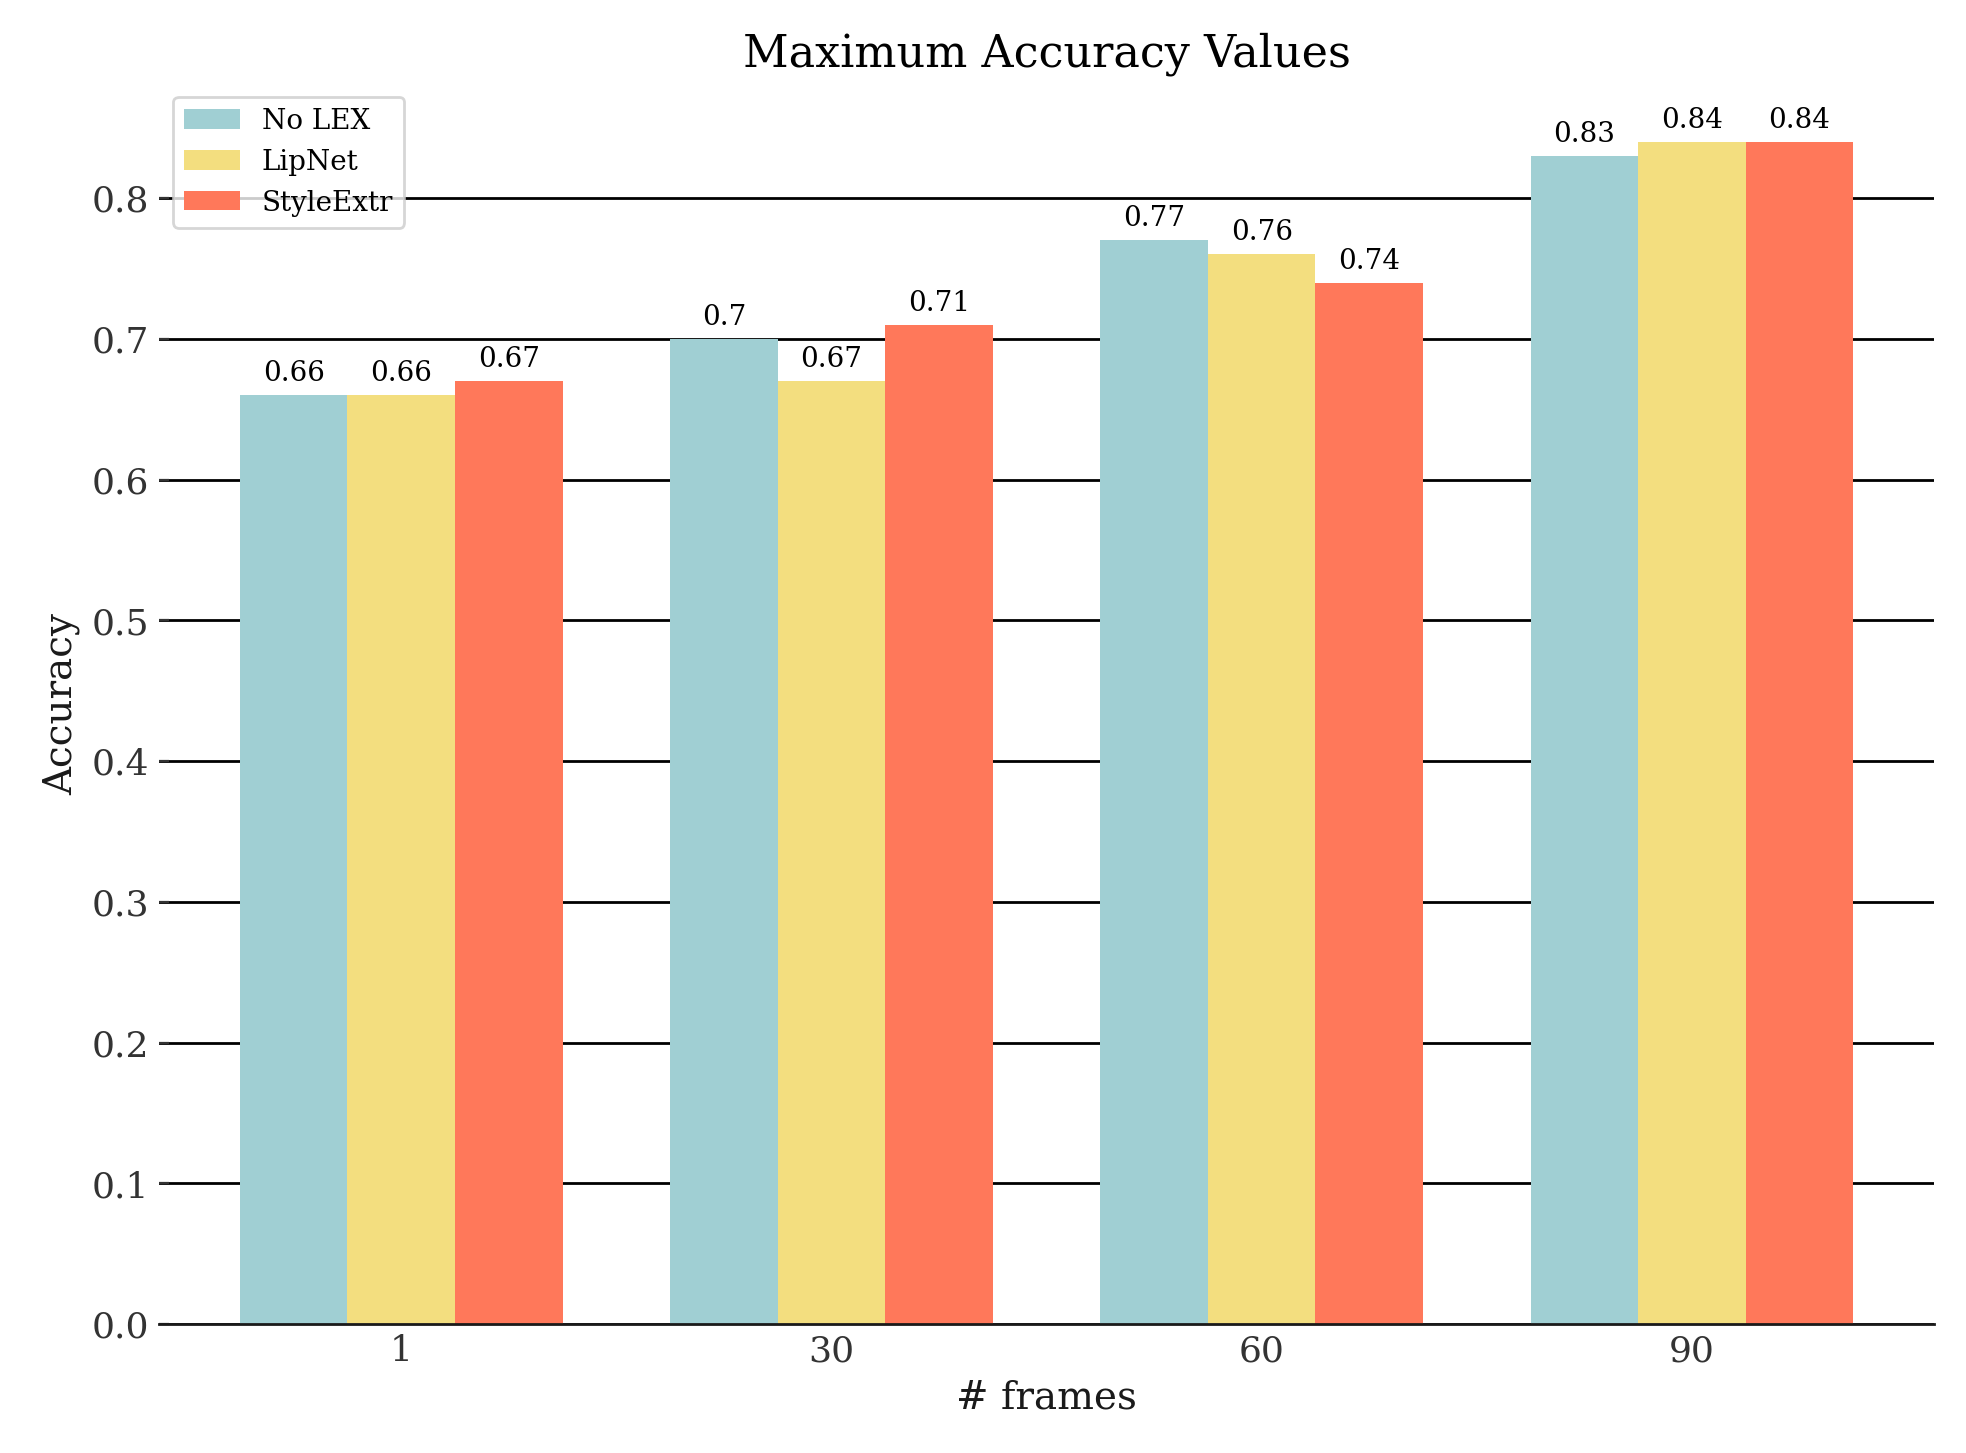
\includegraphics[width=0.8\textwidth]{res/maxaccvalues.png}
    \caption{The maximum validation accuracies during training for our three models. The temporal dimension improves the accuracy, whereas neither lexical compensator shows significant improvements in performance.}
    \label{fig:max_acc}
\end{figure}

\begin{figure}
    \centering
    \begin{subfigure}[b]{0.45\textwidth}
      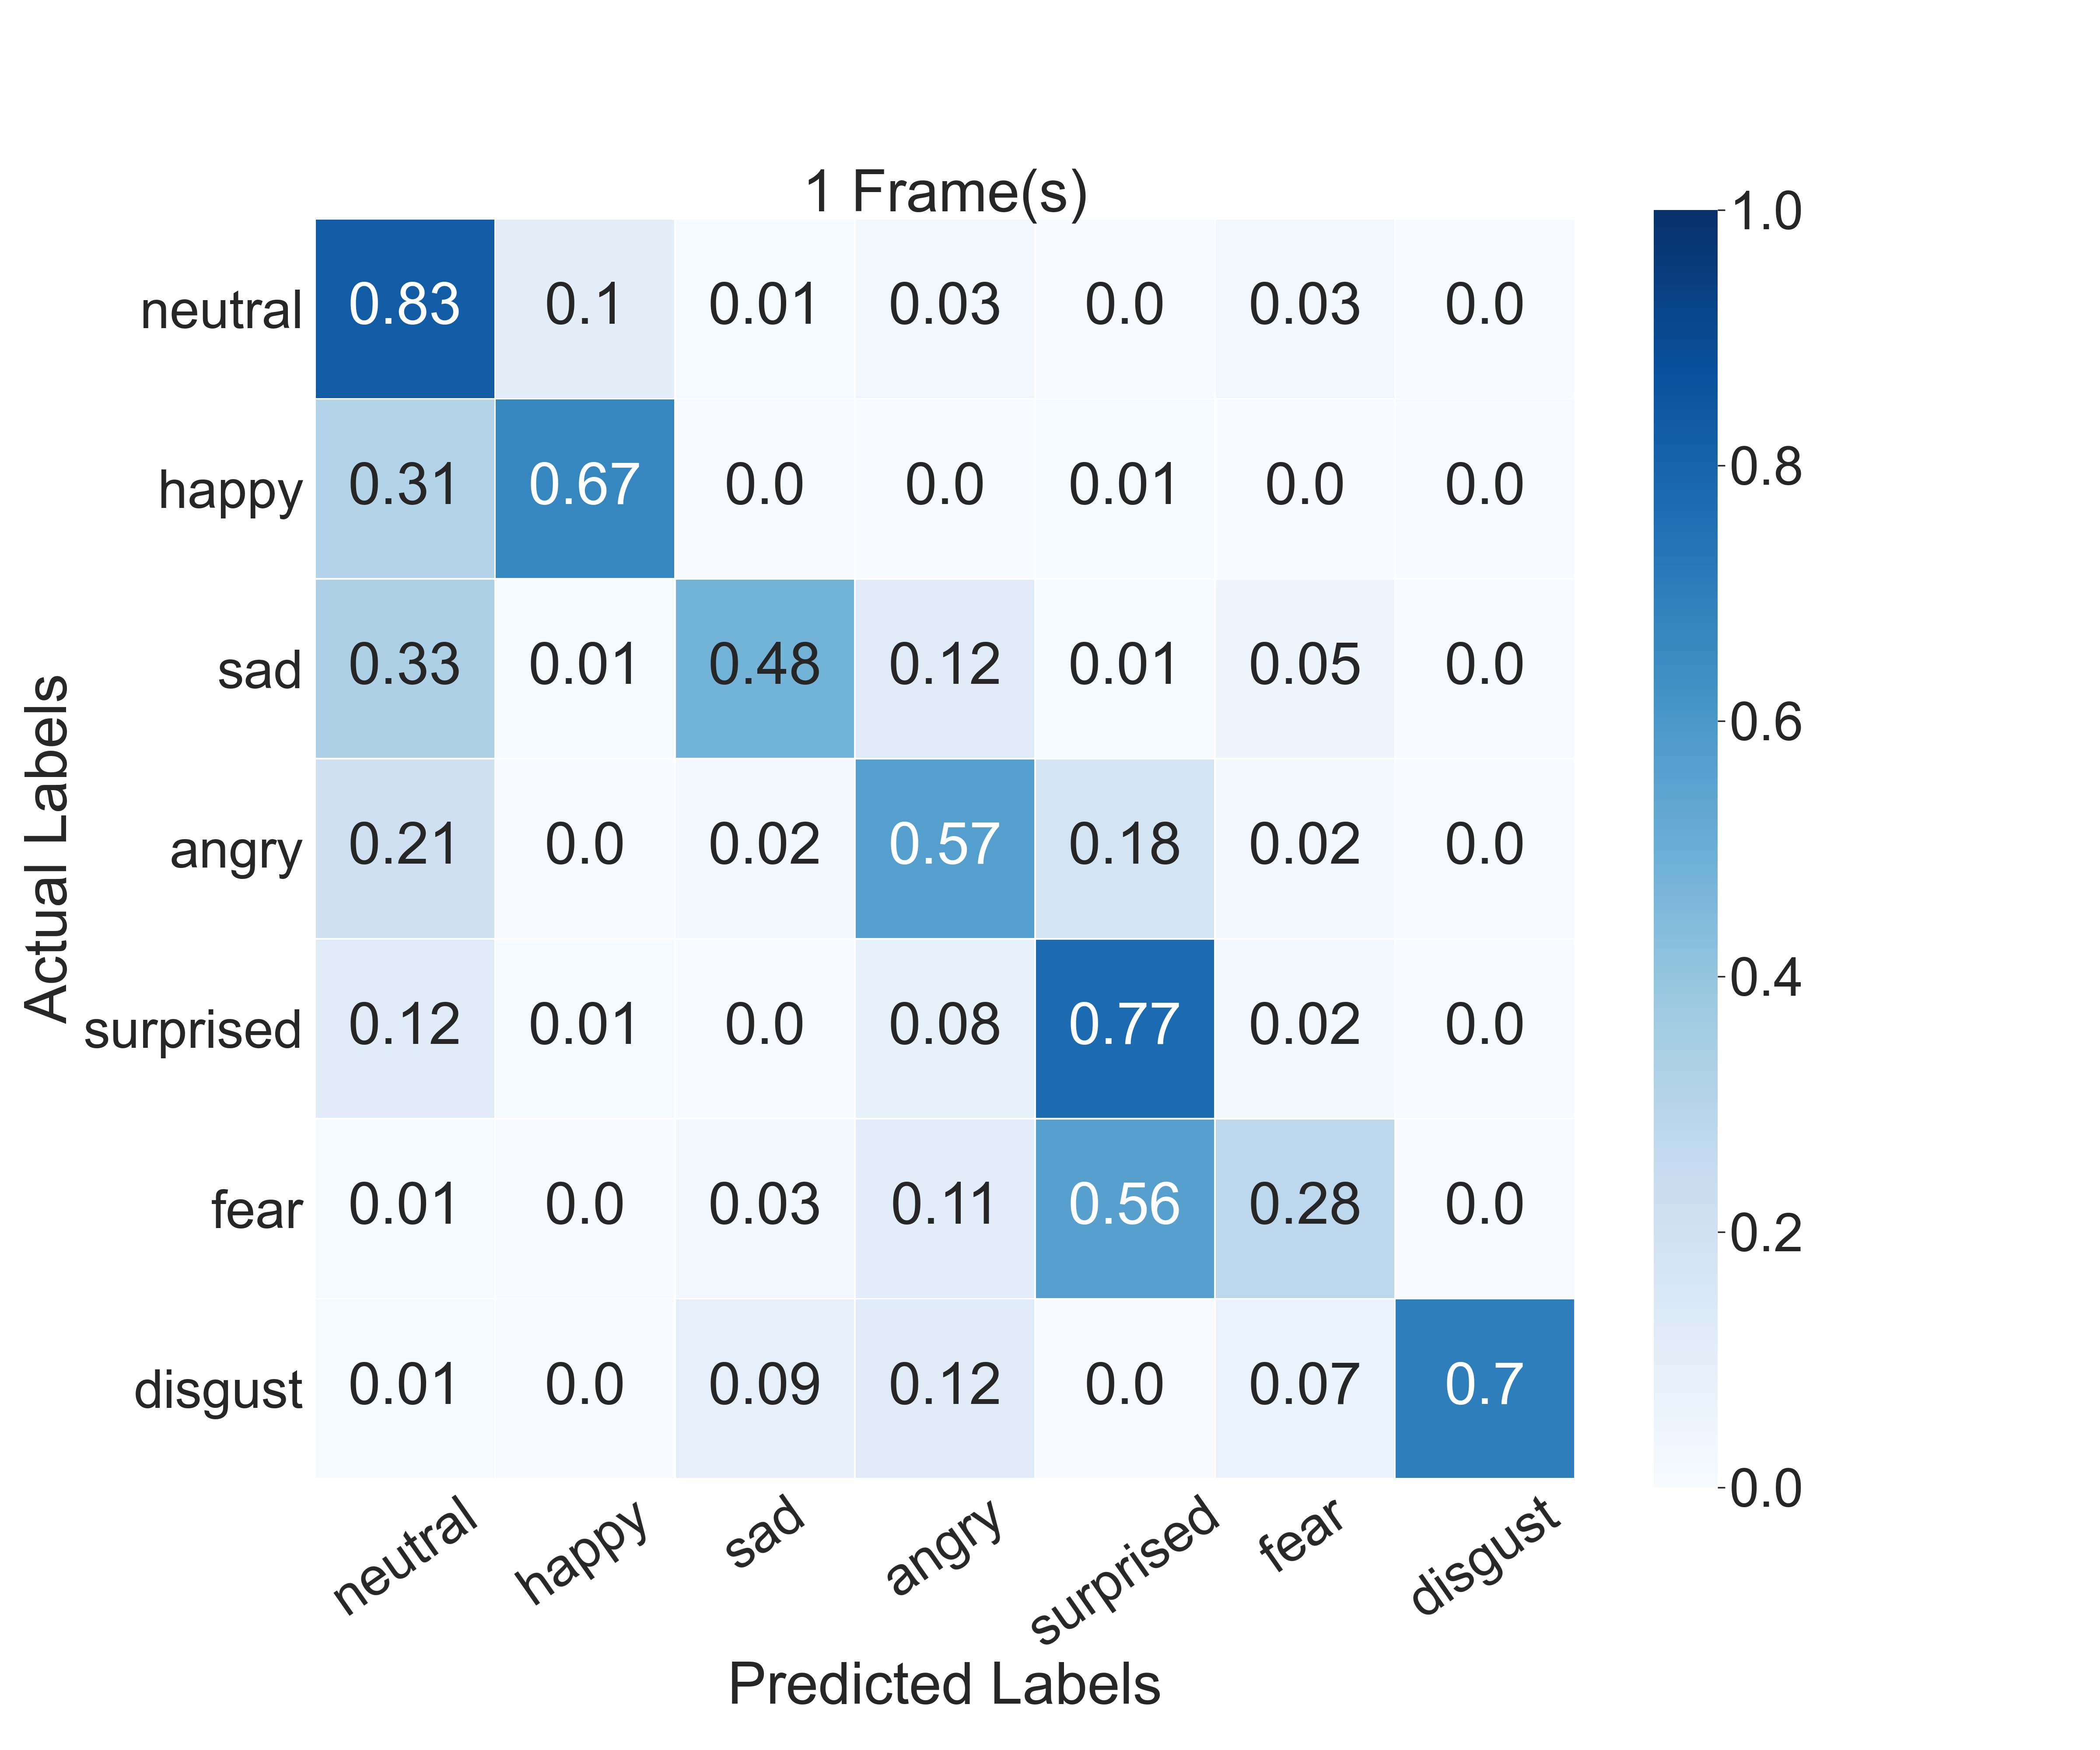
\includegraphics[width=\textwidth]{res/conf_fer_1.png}
    \end{subfigure}
    \begin{subfigure}[b]{0.45\textwidth}
      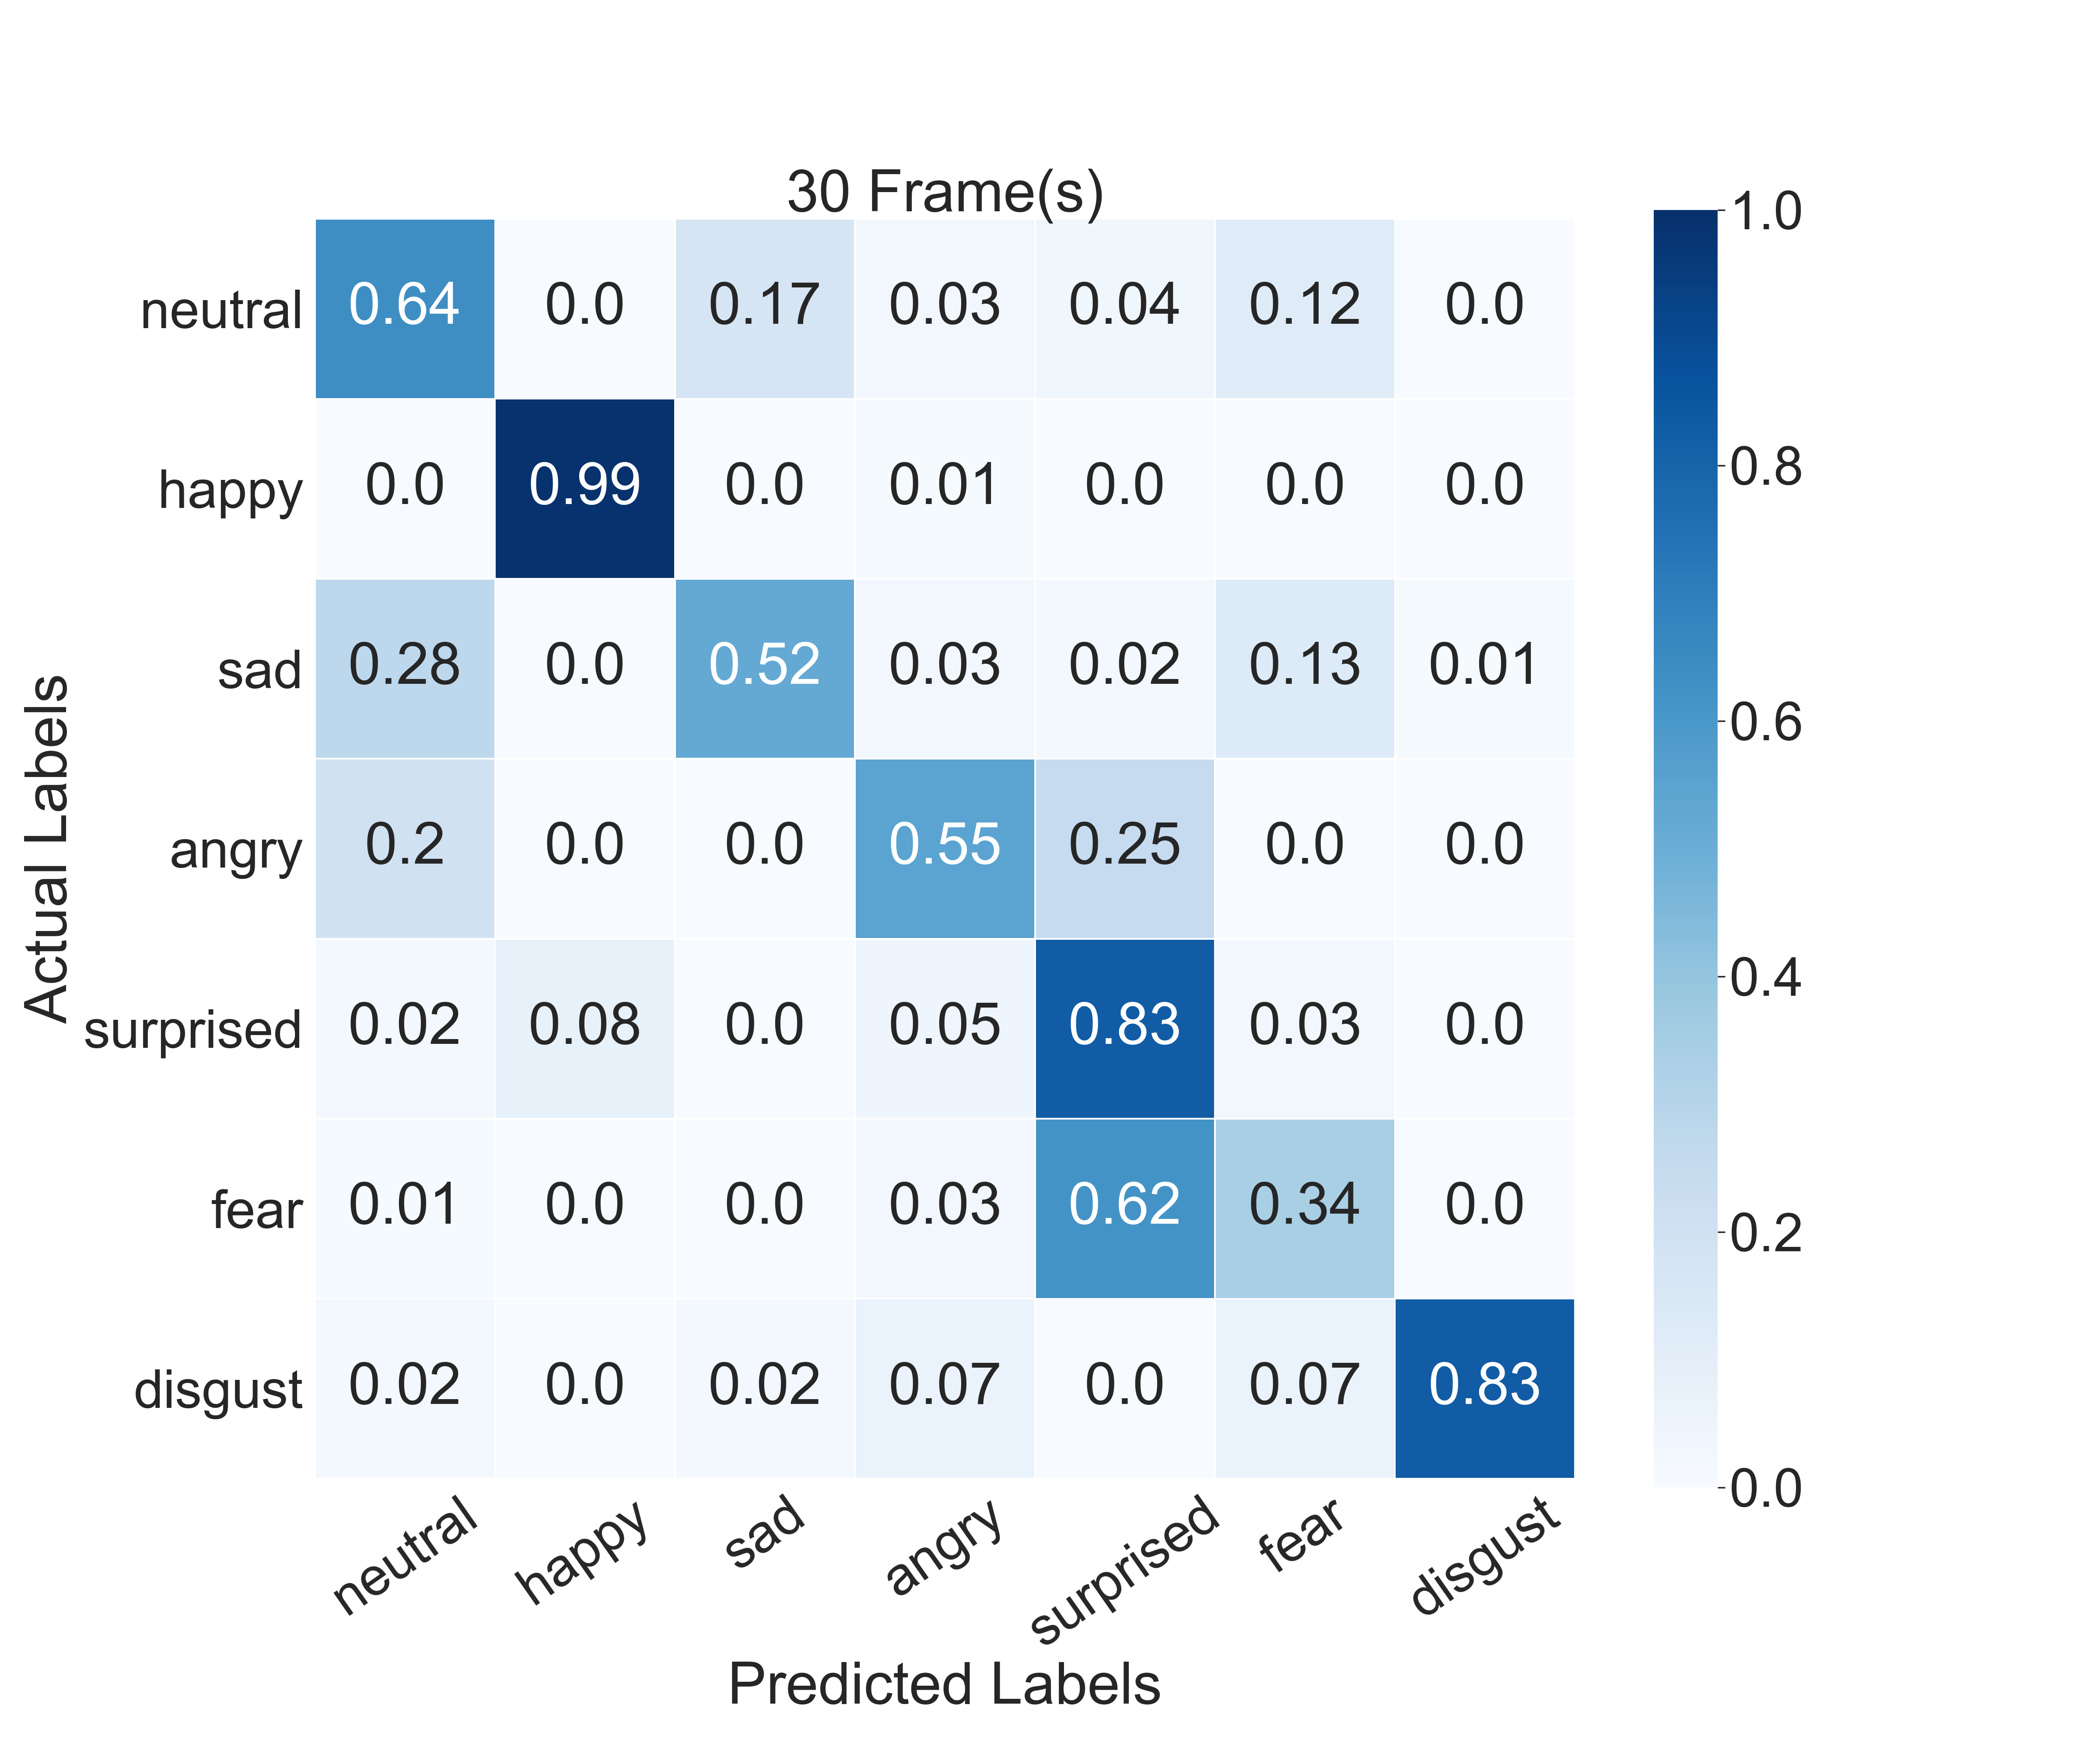
\includegraphics[width=\textwidth]{res/conf_fer_30.png}
    \end{subfigure}
    \begin{subfigure}[b]{0.45\textwidth}
      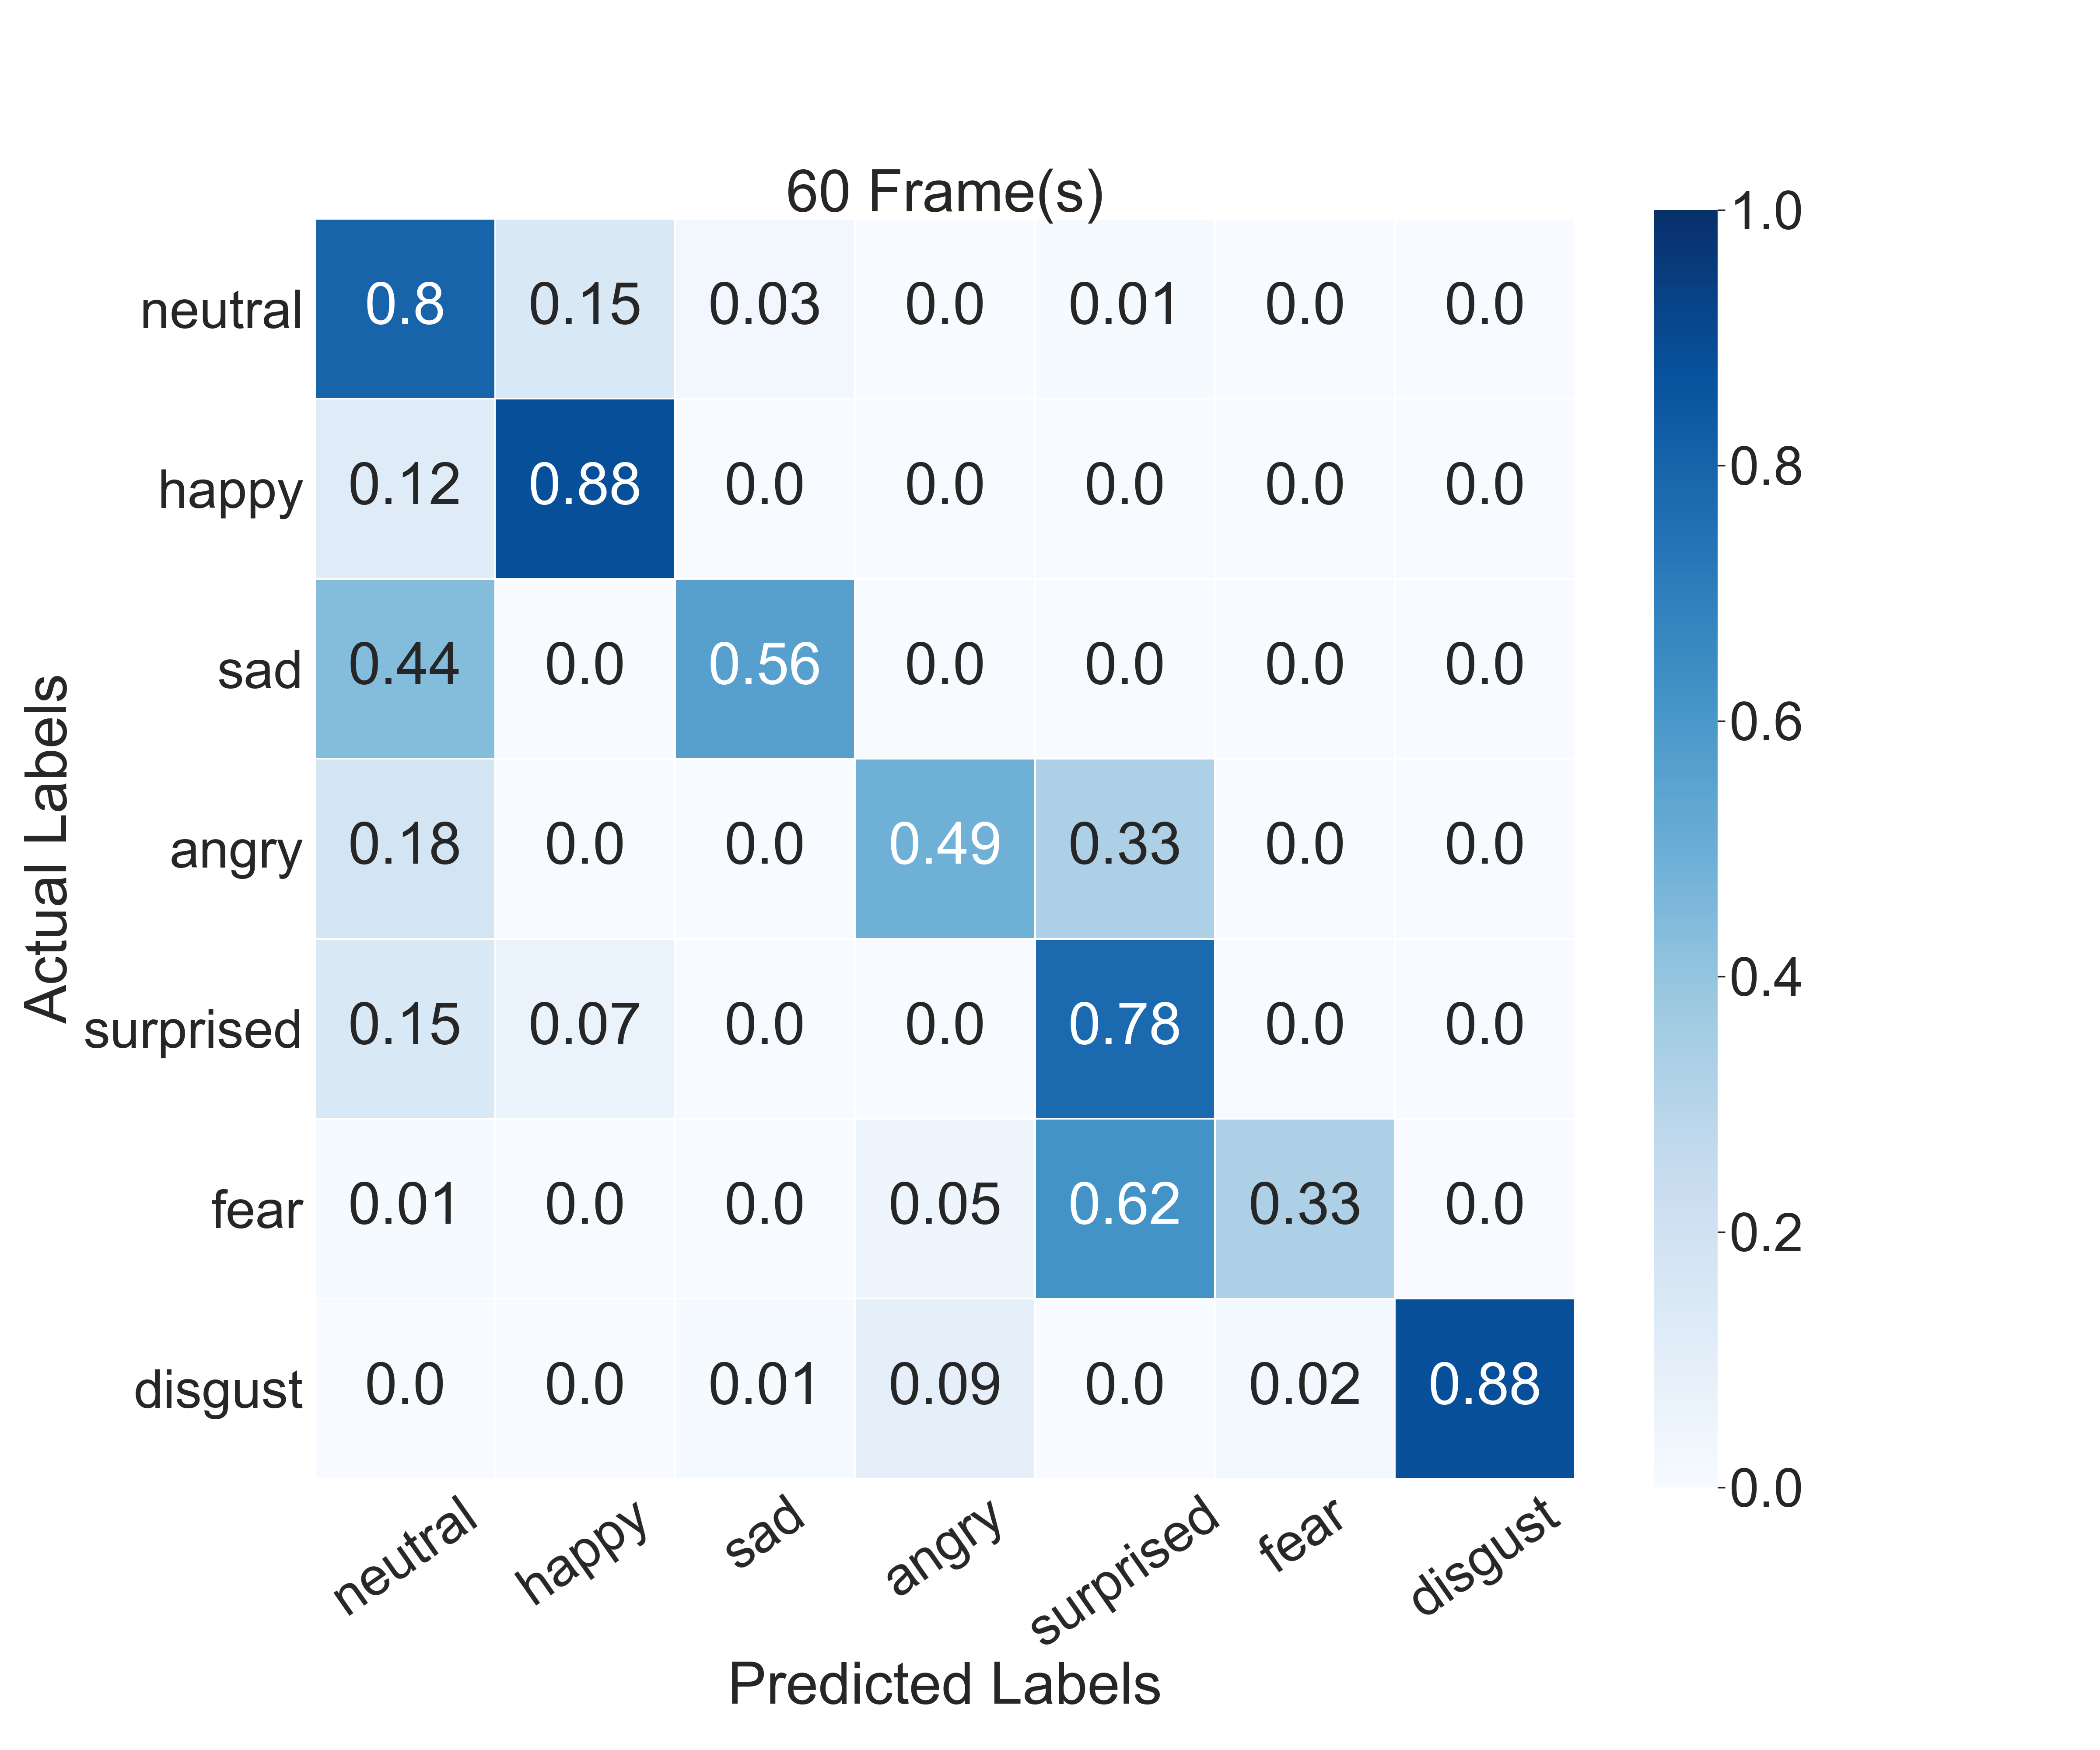
\includegraphics[width=\textwidth]{res/conf_fer_60.png}
    \end{subfigure}
    \begin{subfigure}[b]{0.45\textwidth}
      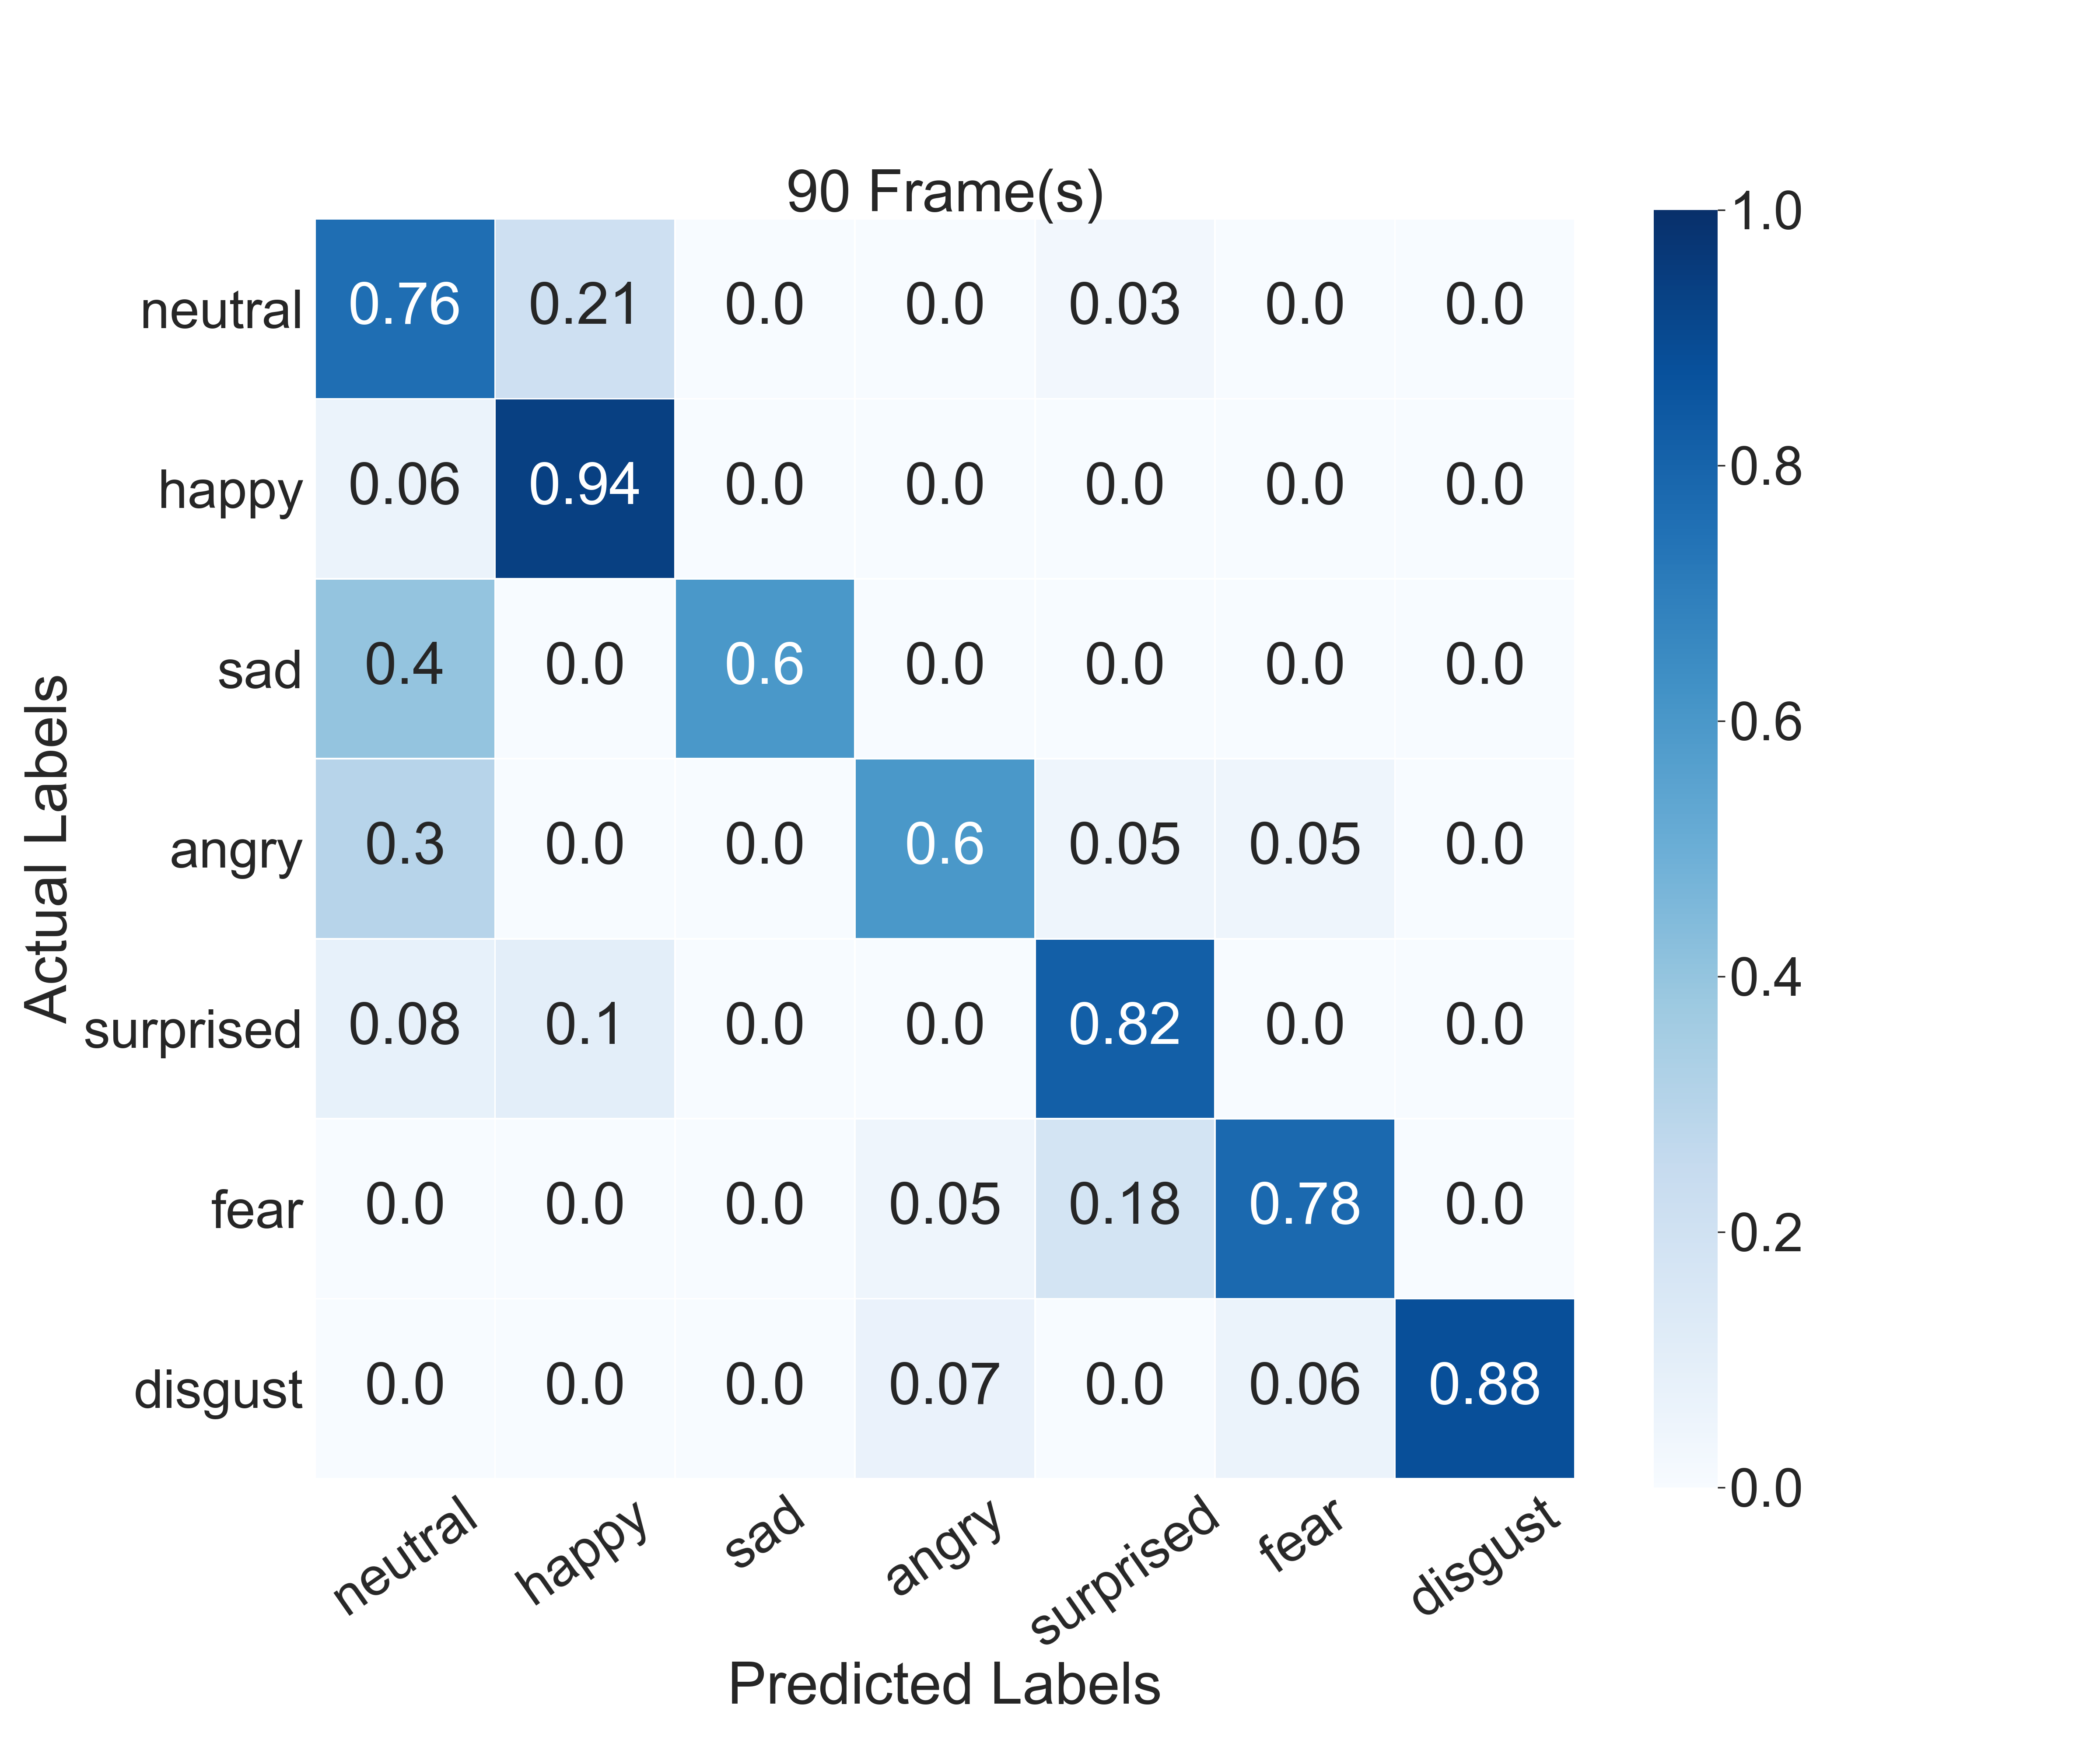
\includegraphics[width=\textwidth]{res/conf_fer_90.png}
    \end{subfigure}
    \caption{Confusion matrices of the validation data for the FER model without a lexical compensator.}
    \label{fig:fer_conf}
\end{figure}

\begin{figure}
    \centering
    \begin{subfigure}[b]{0.45\textwidth}
      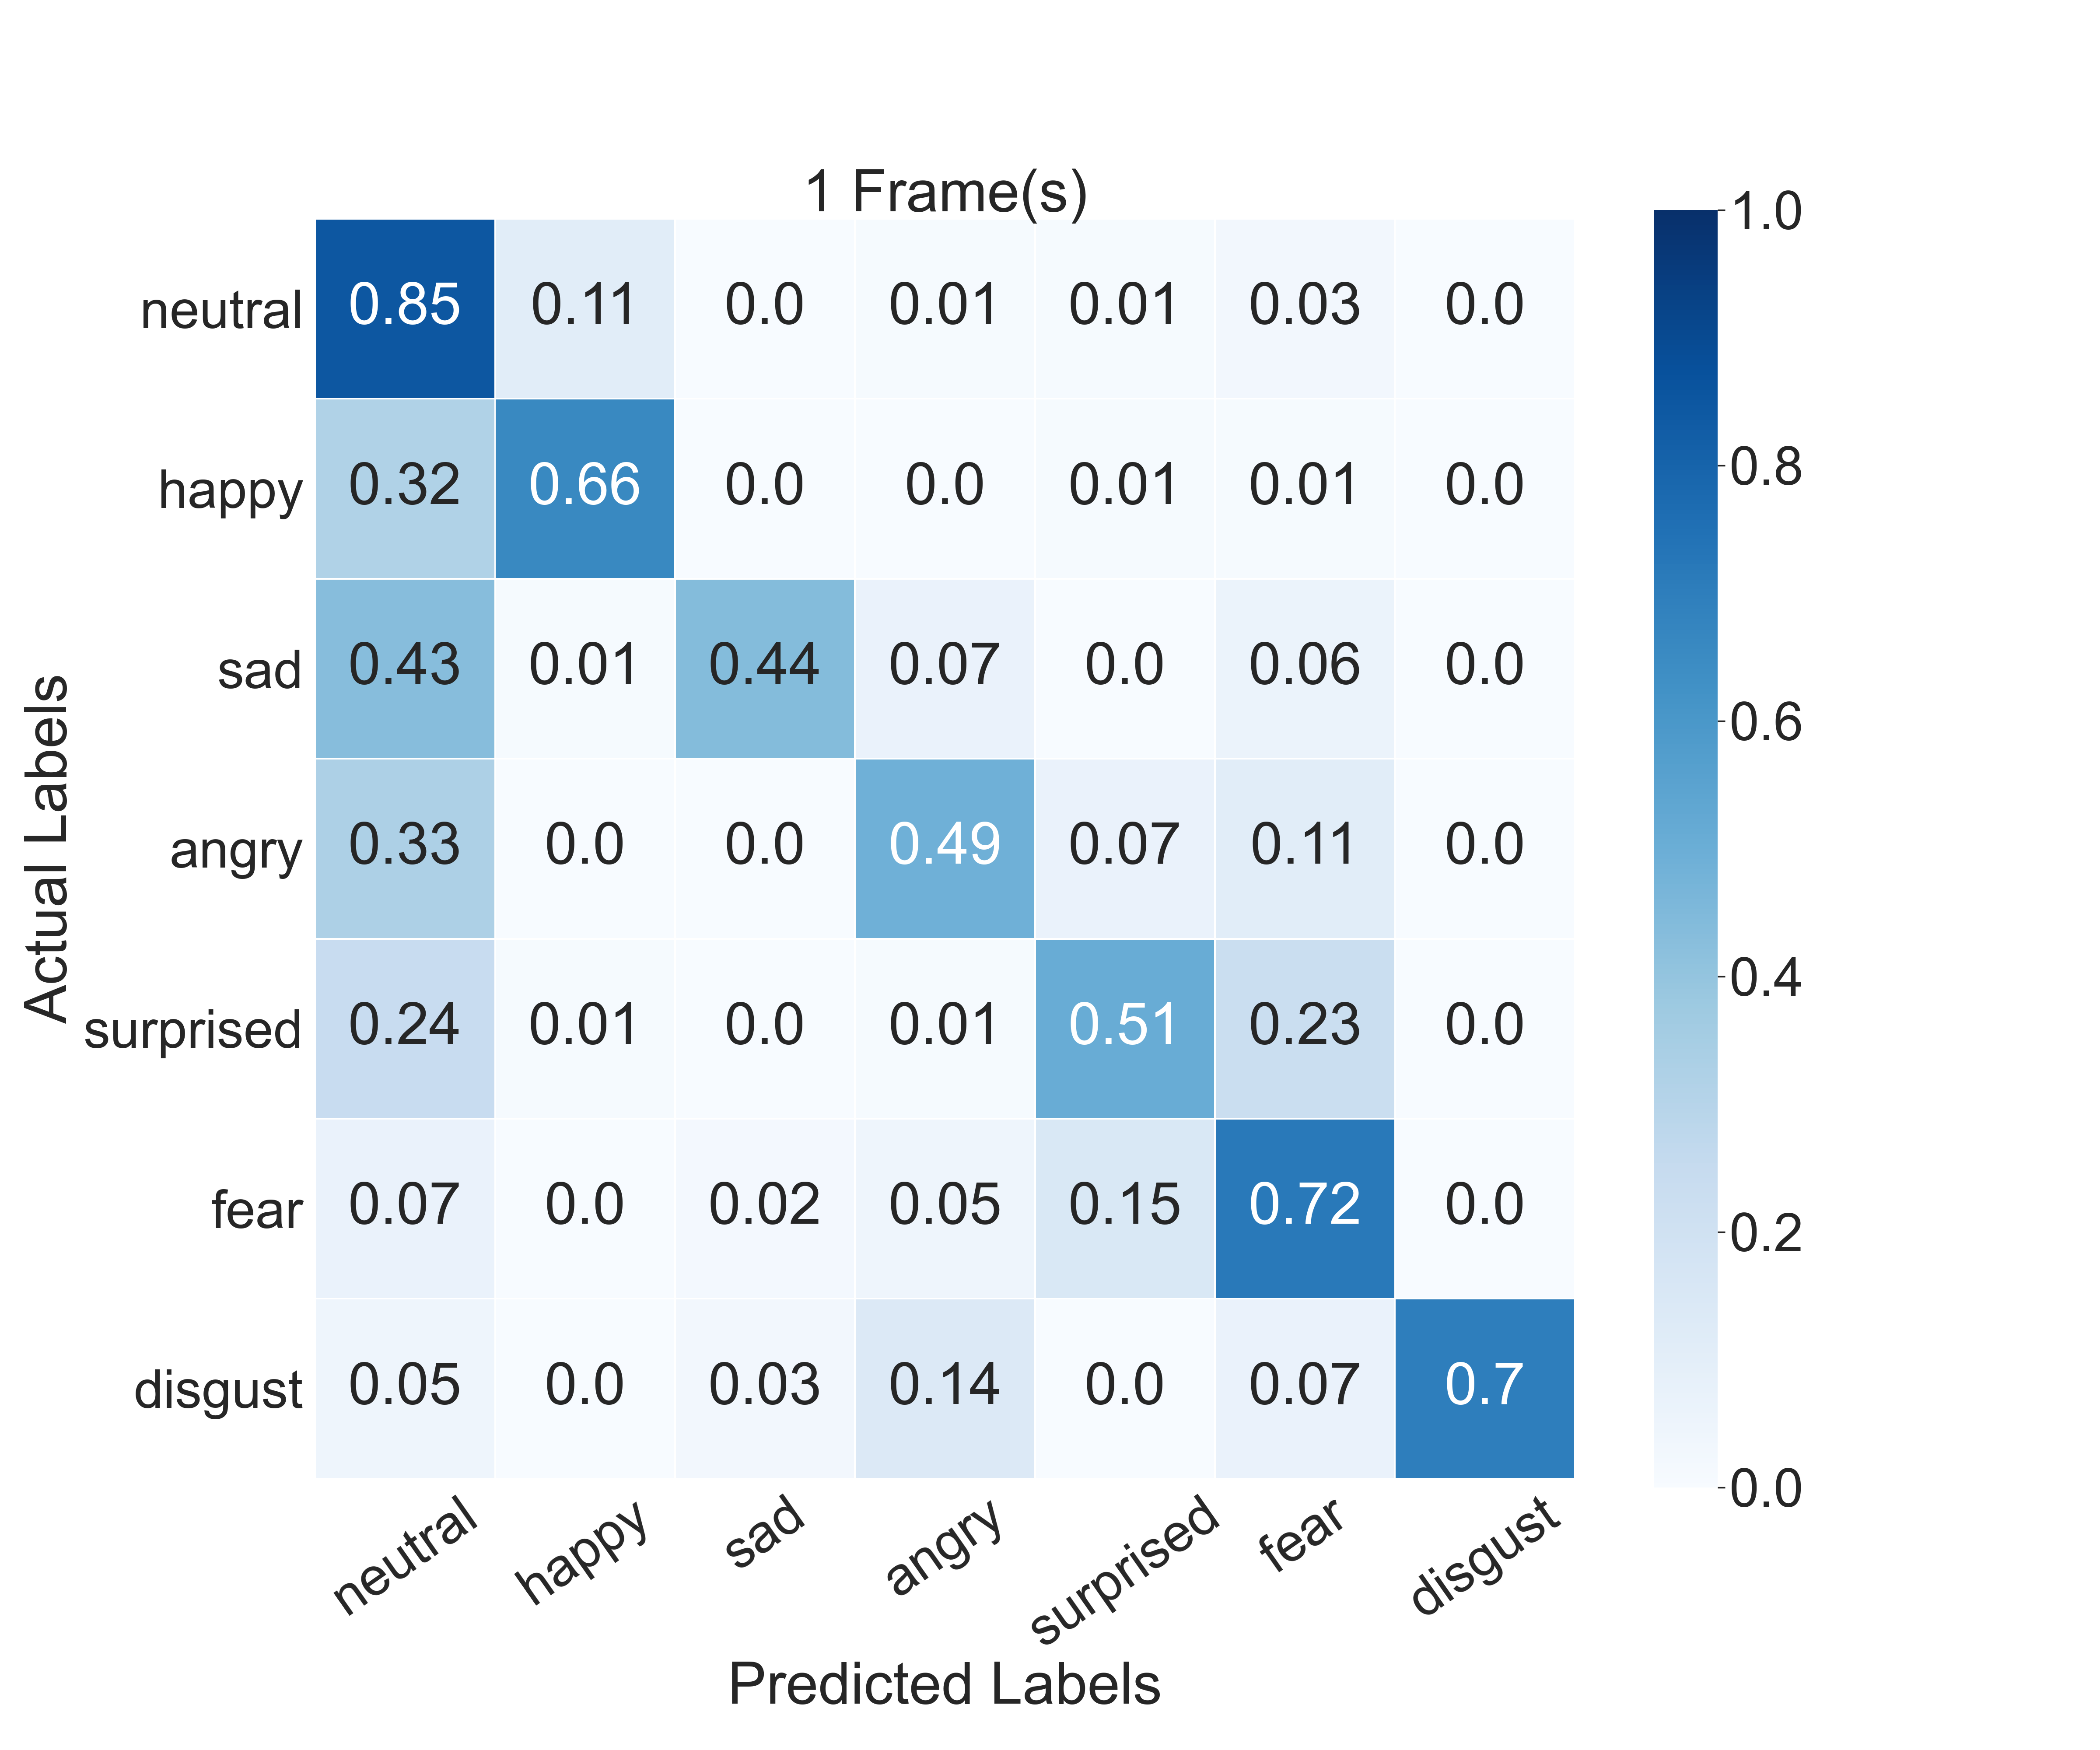
\includegraphics[width=\textwidth]{res/conf_fusion_1.png}
    \end{subfigure}
    \begin{subfigure}[b]{0.45\textwidth}
      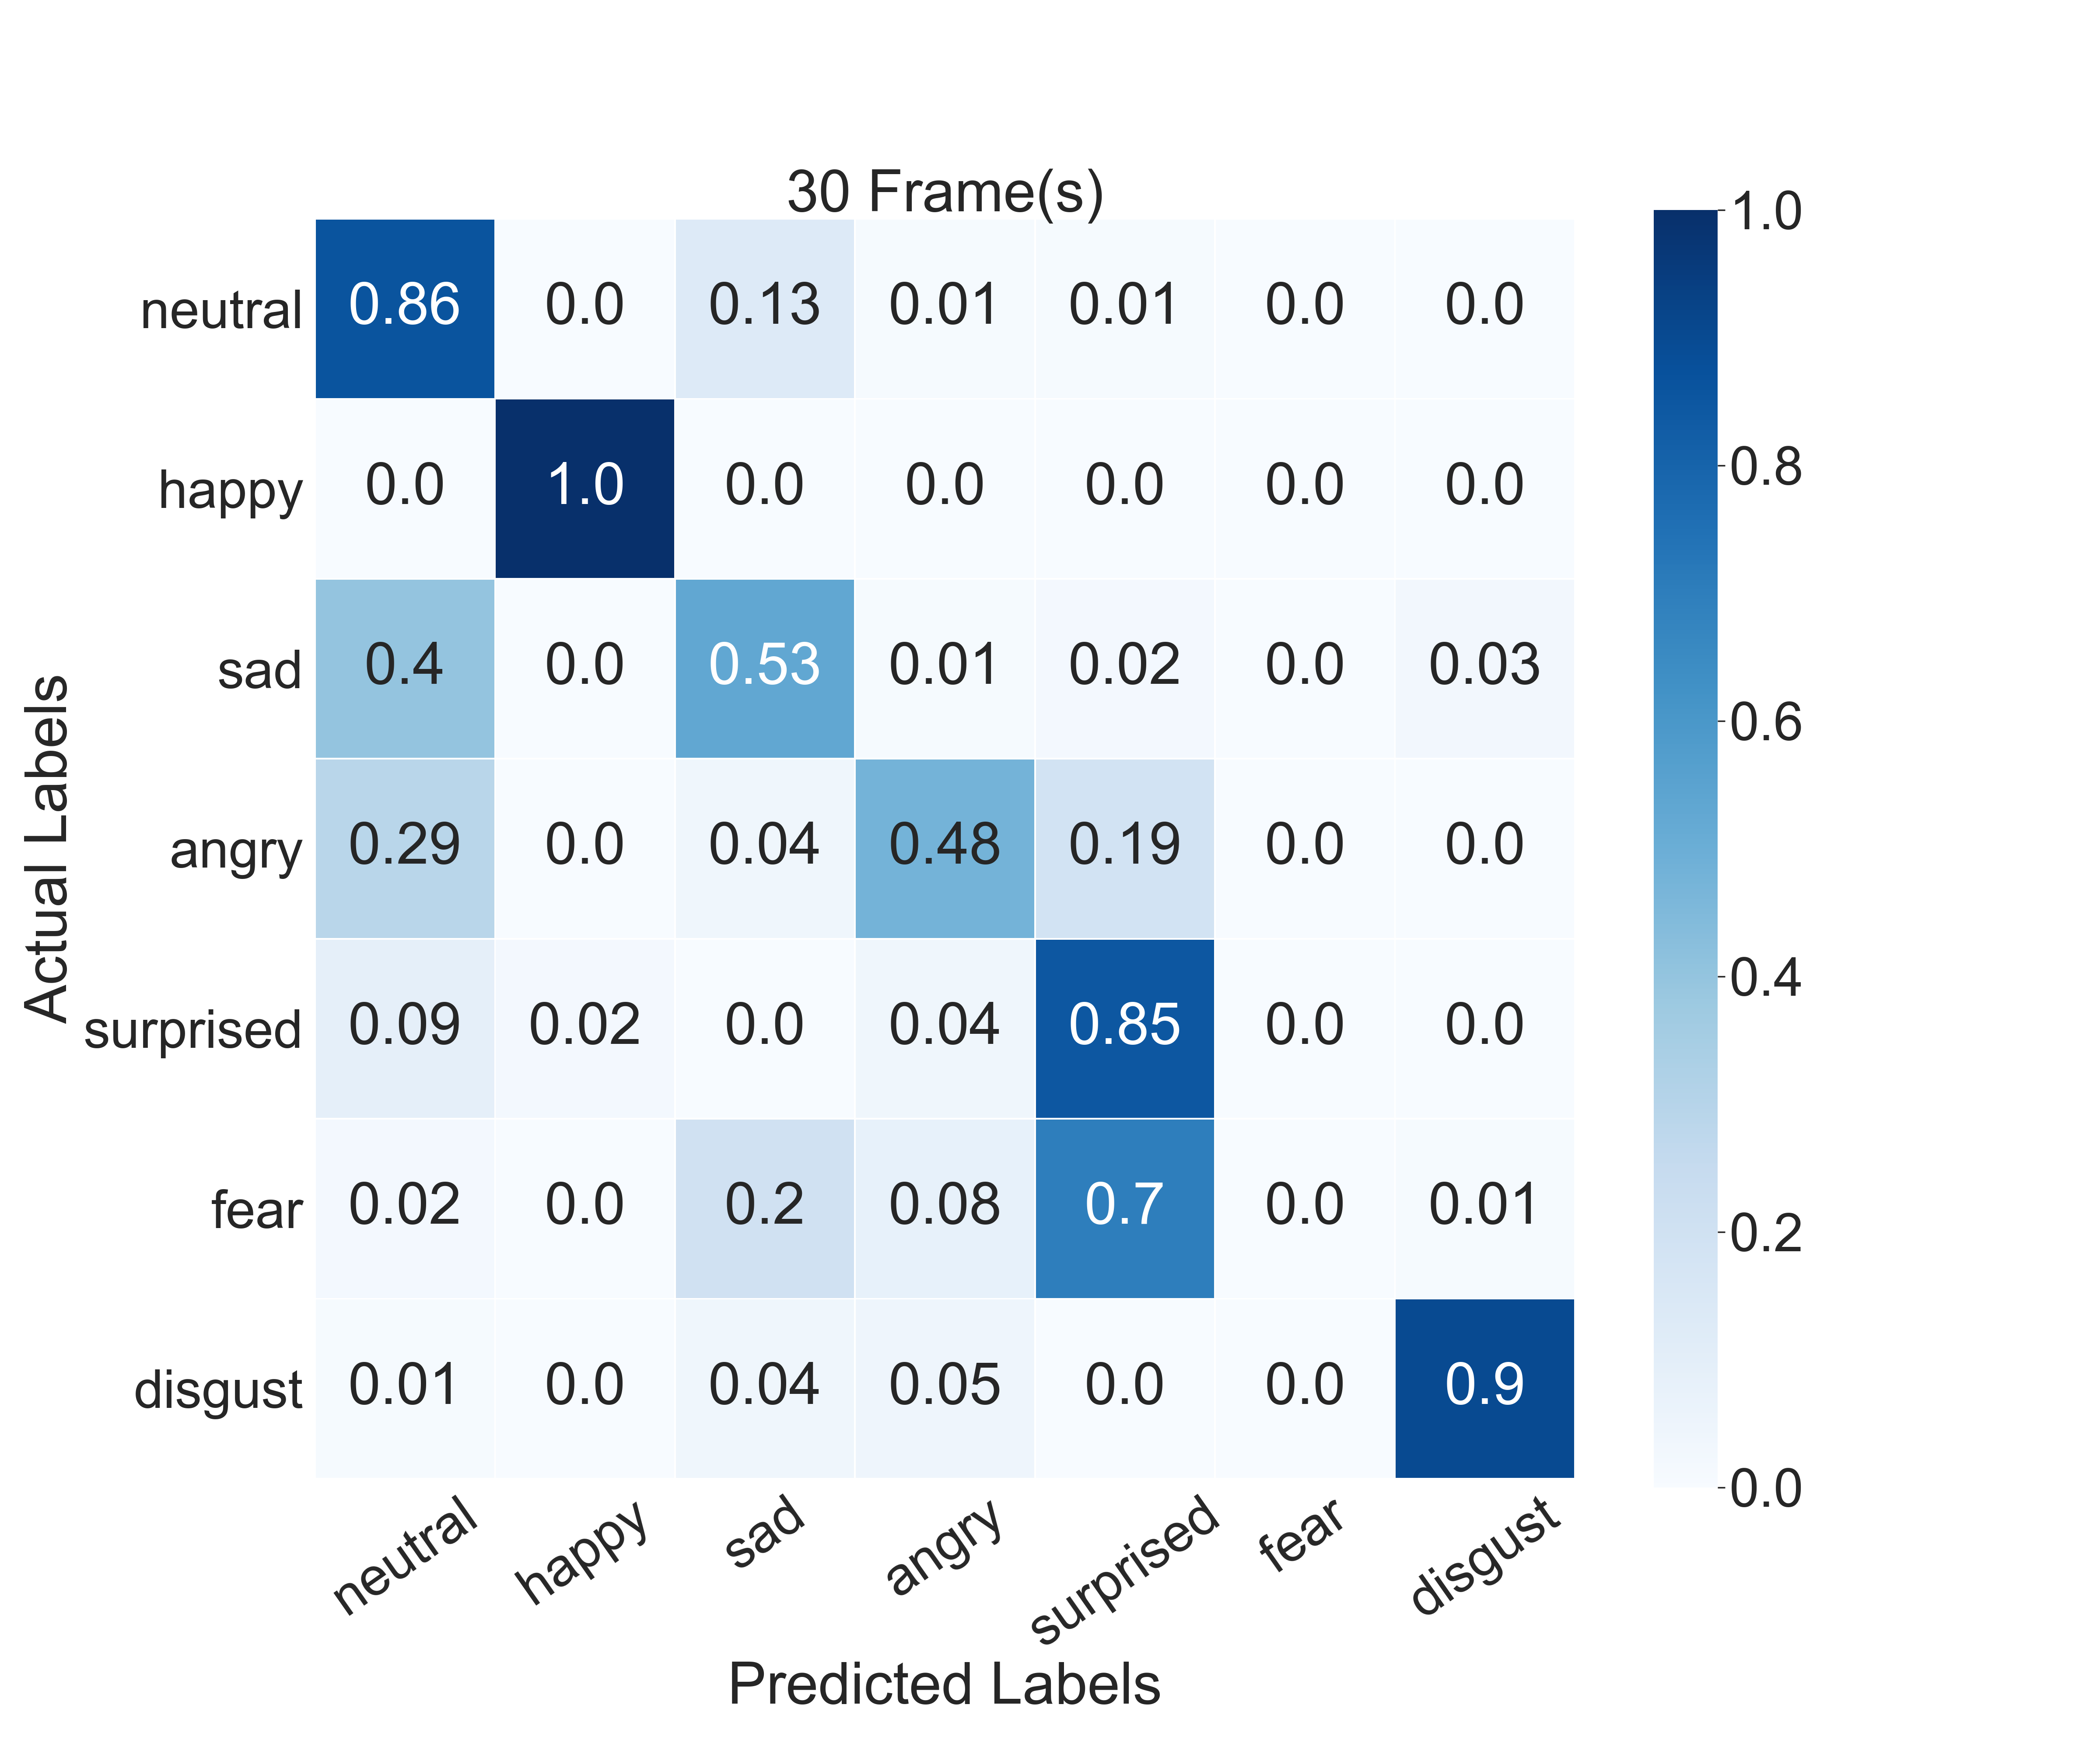
\includegraphics[width=\textwidth]{res/conf_fusion_30.png}
    \end{subfigure}
    \begin{subfigure}[b]{0.45\textwidth}
      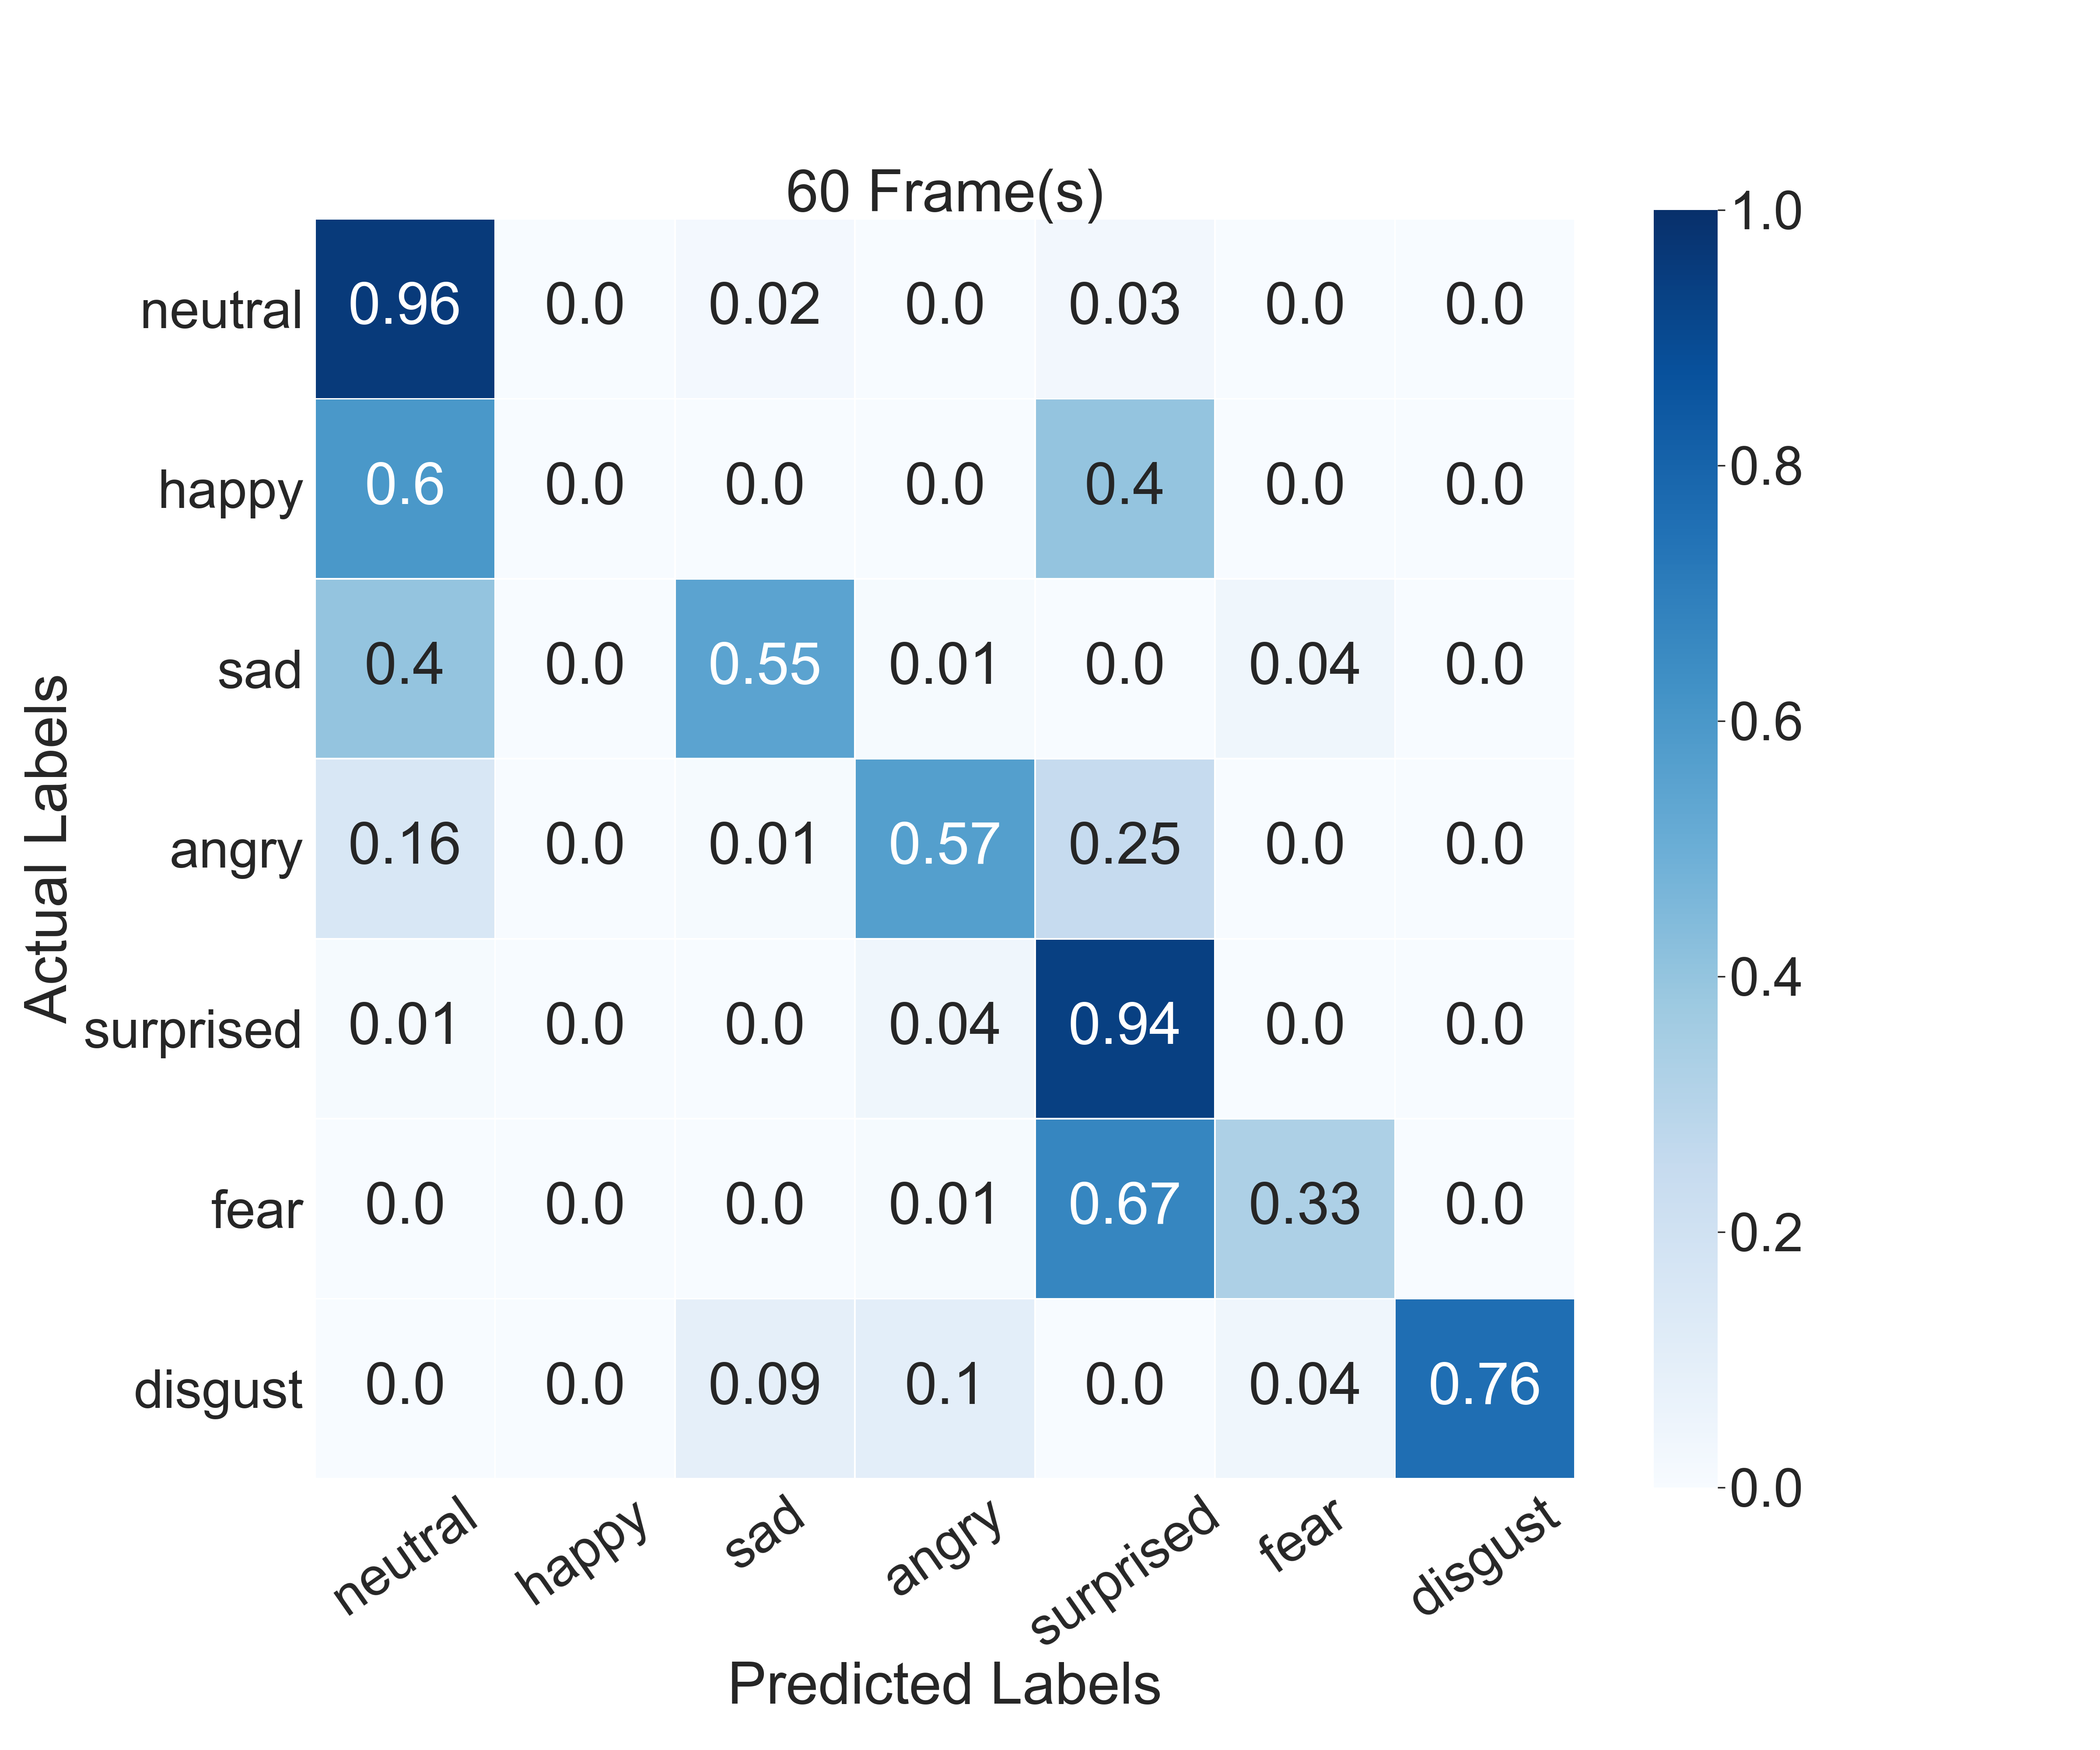
\includegraphics[width=\textwidth]{res/conf_fusion_60.png}
    \end{subfigure}
    \begin{subfigure}[b]{0.45\textwidth}
      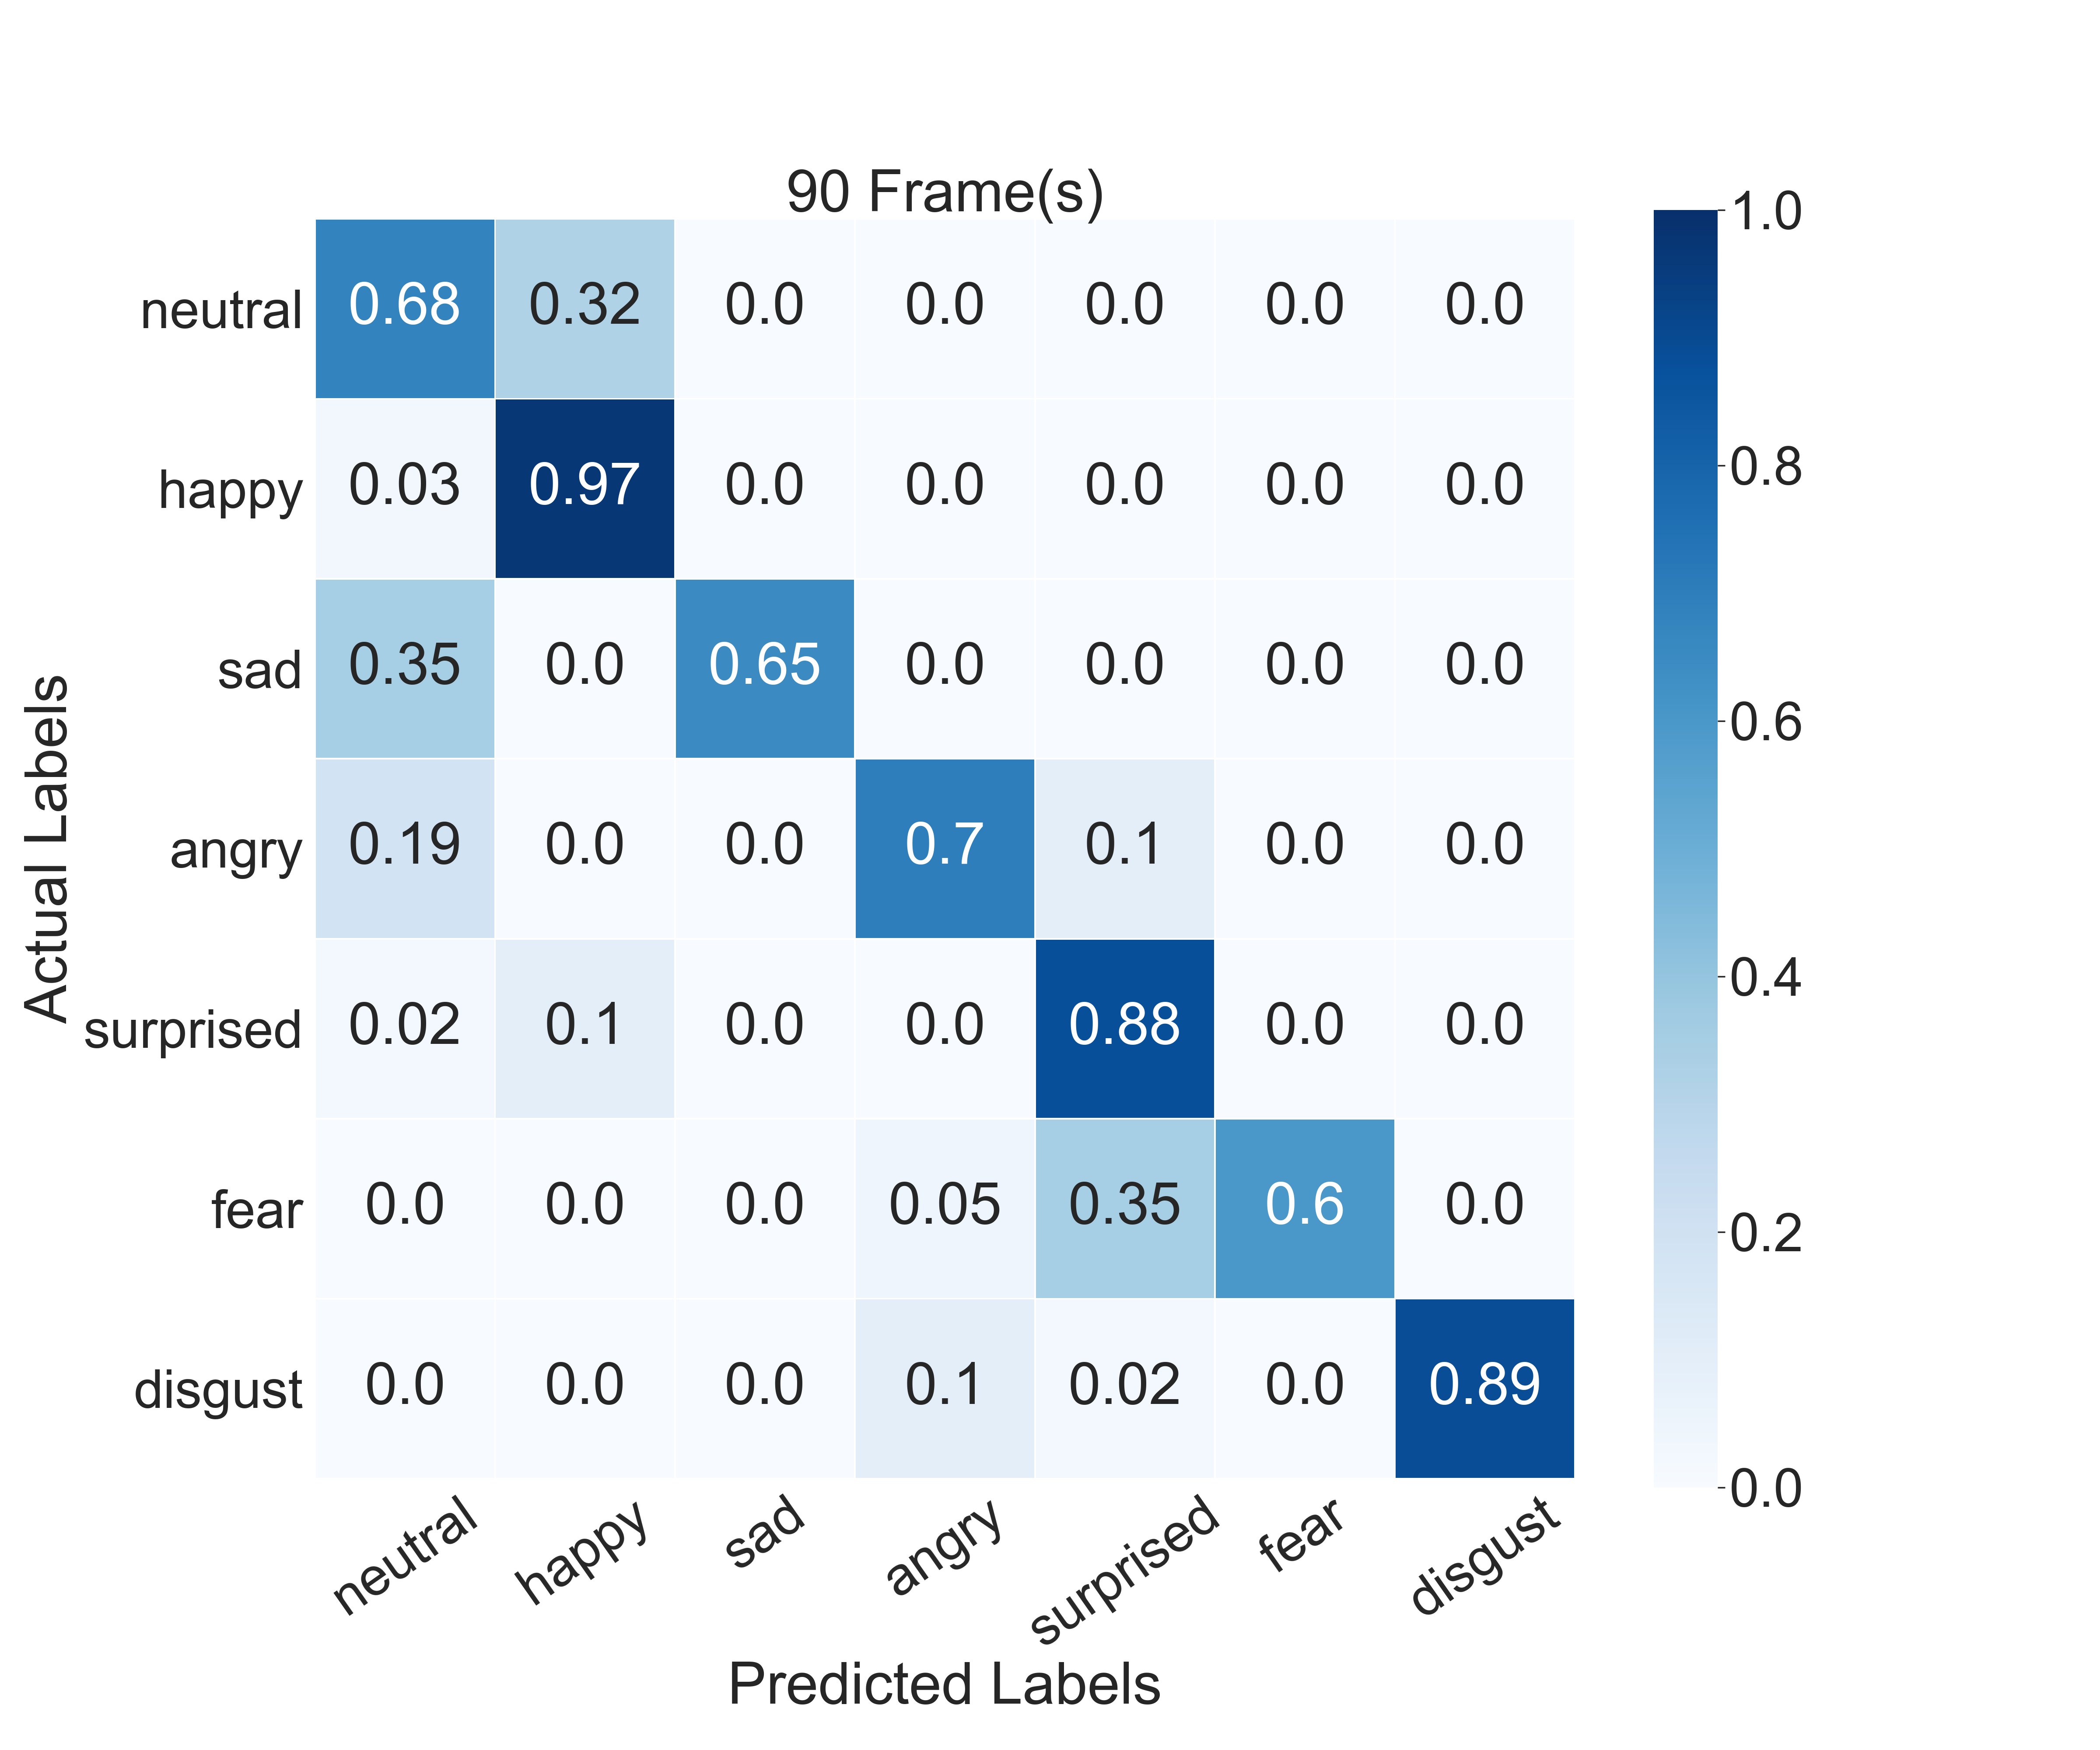
\includegraphics[width=\textwidth]{res/conf_fusion_90.png}
    \end{subfigure}
    \caption{Confusion matrices of the validation data for the LipNet fusion model.}
    \label{fig:lipnet_conf}
\end{figure}
\begin{figure}
    \centering
    \begin{subfigure}[b]{0.45\textwidth}
      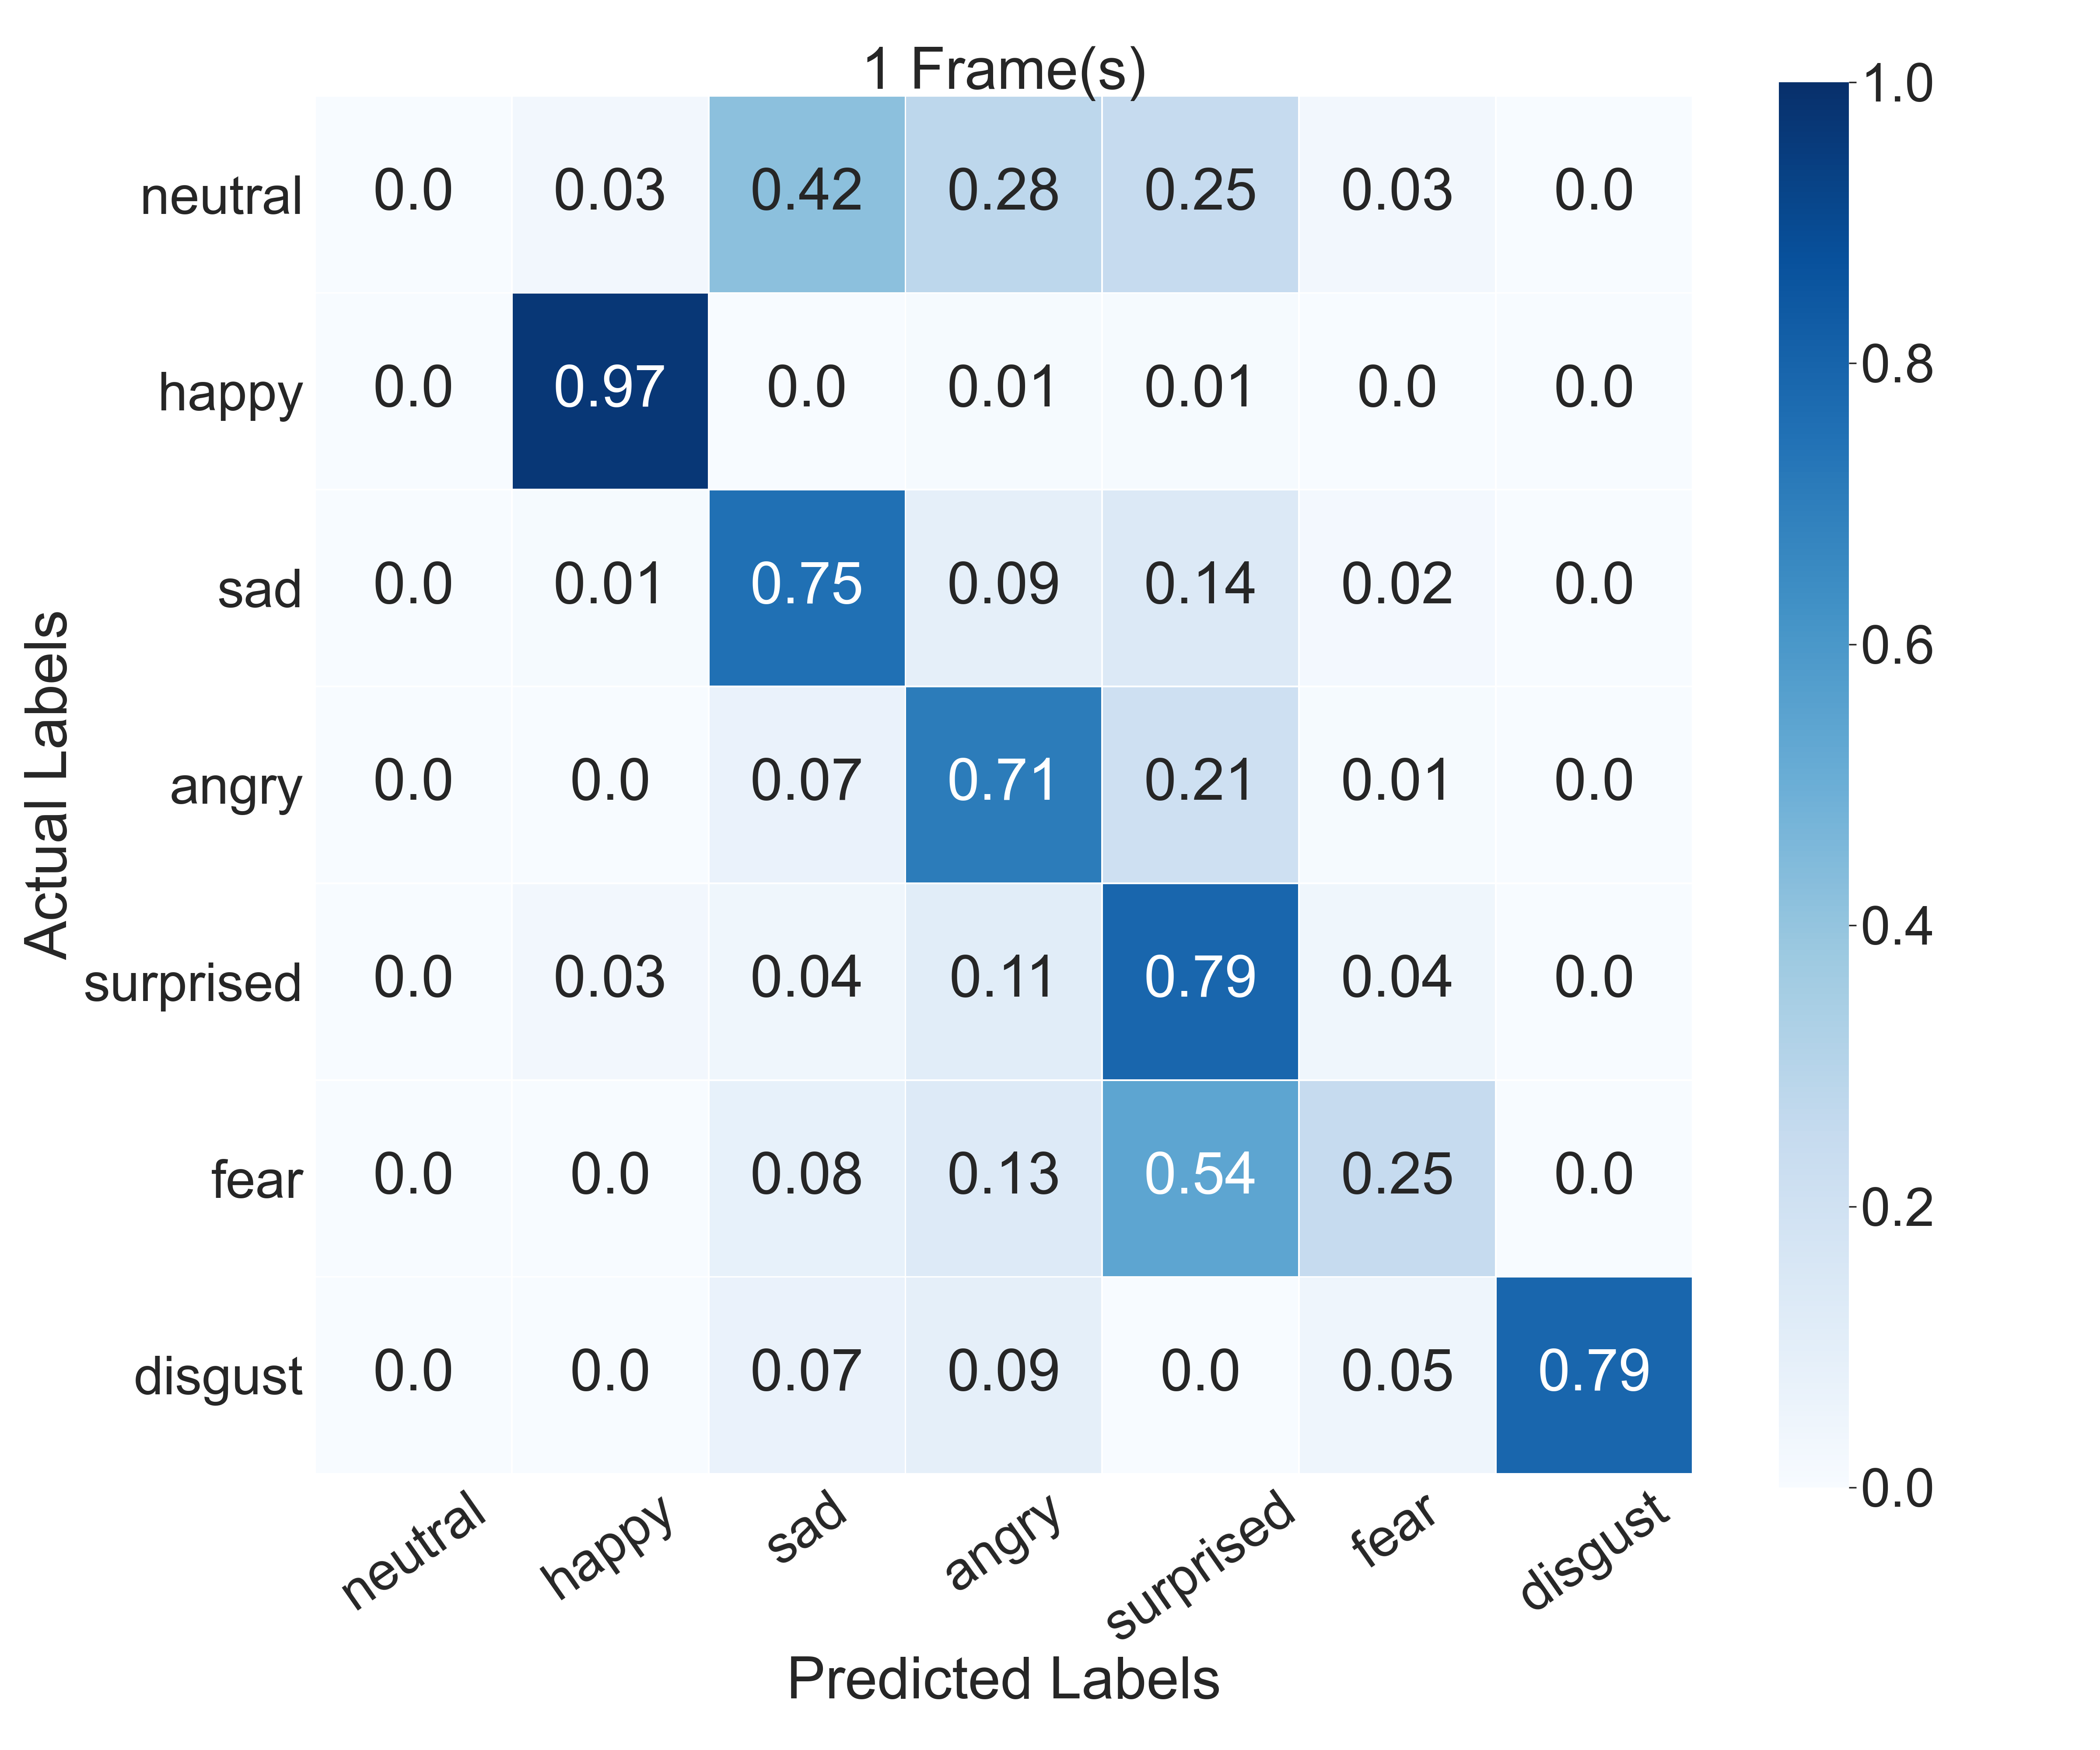
\includegraphics[width=\textwidth]{res/conf_busso_1.png}
    \end{subfigure}
    \begin{subfigure}[b]{0.45\textwidth}
      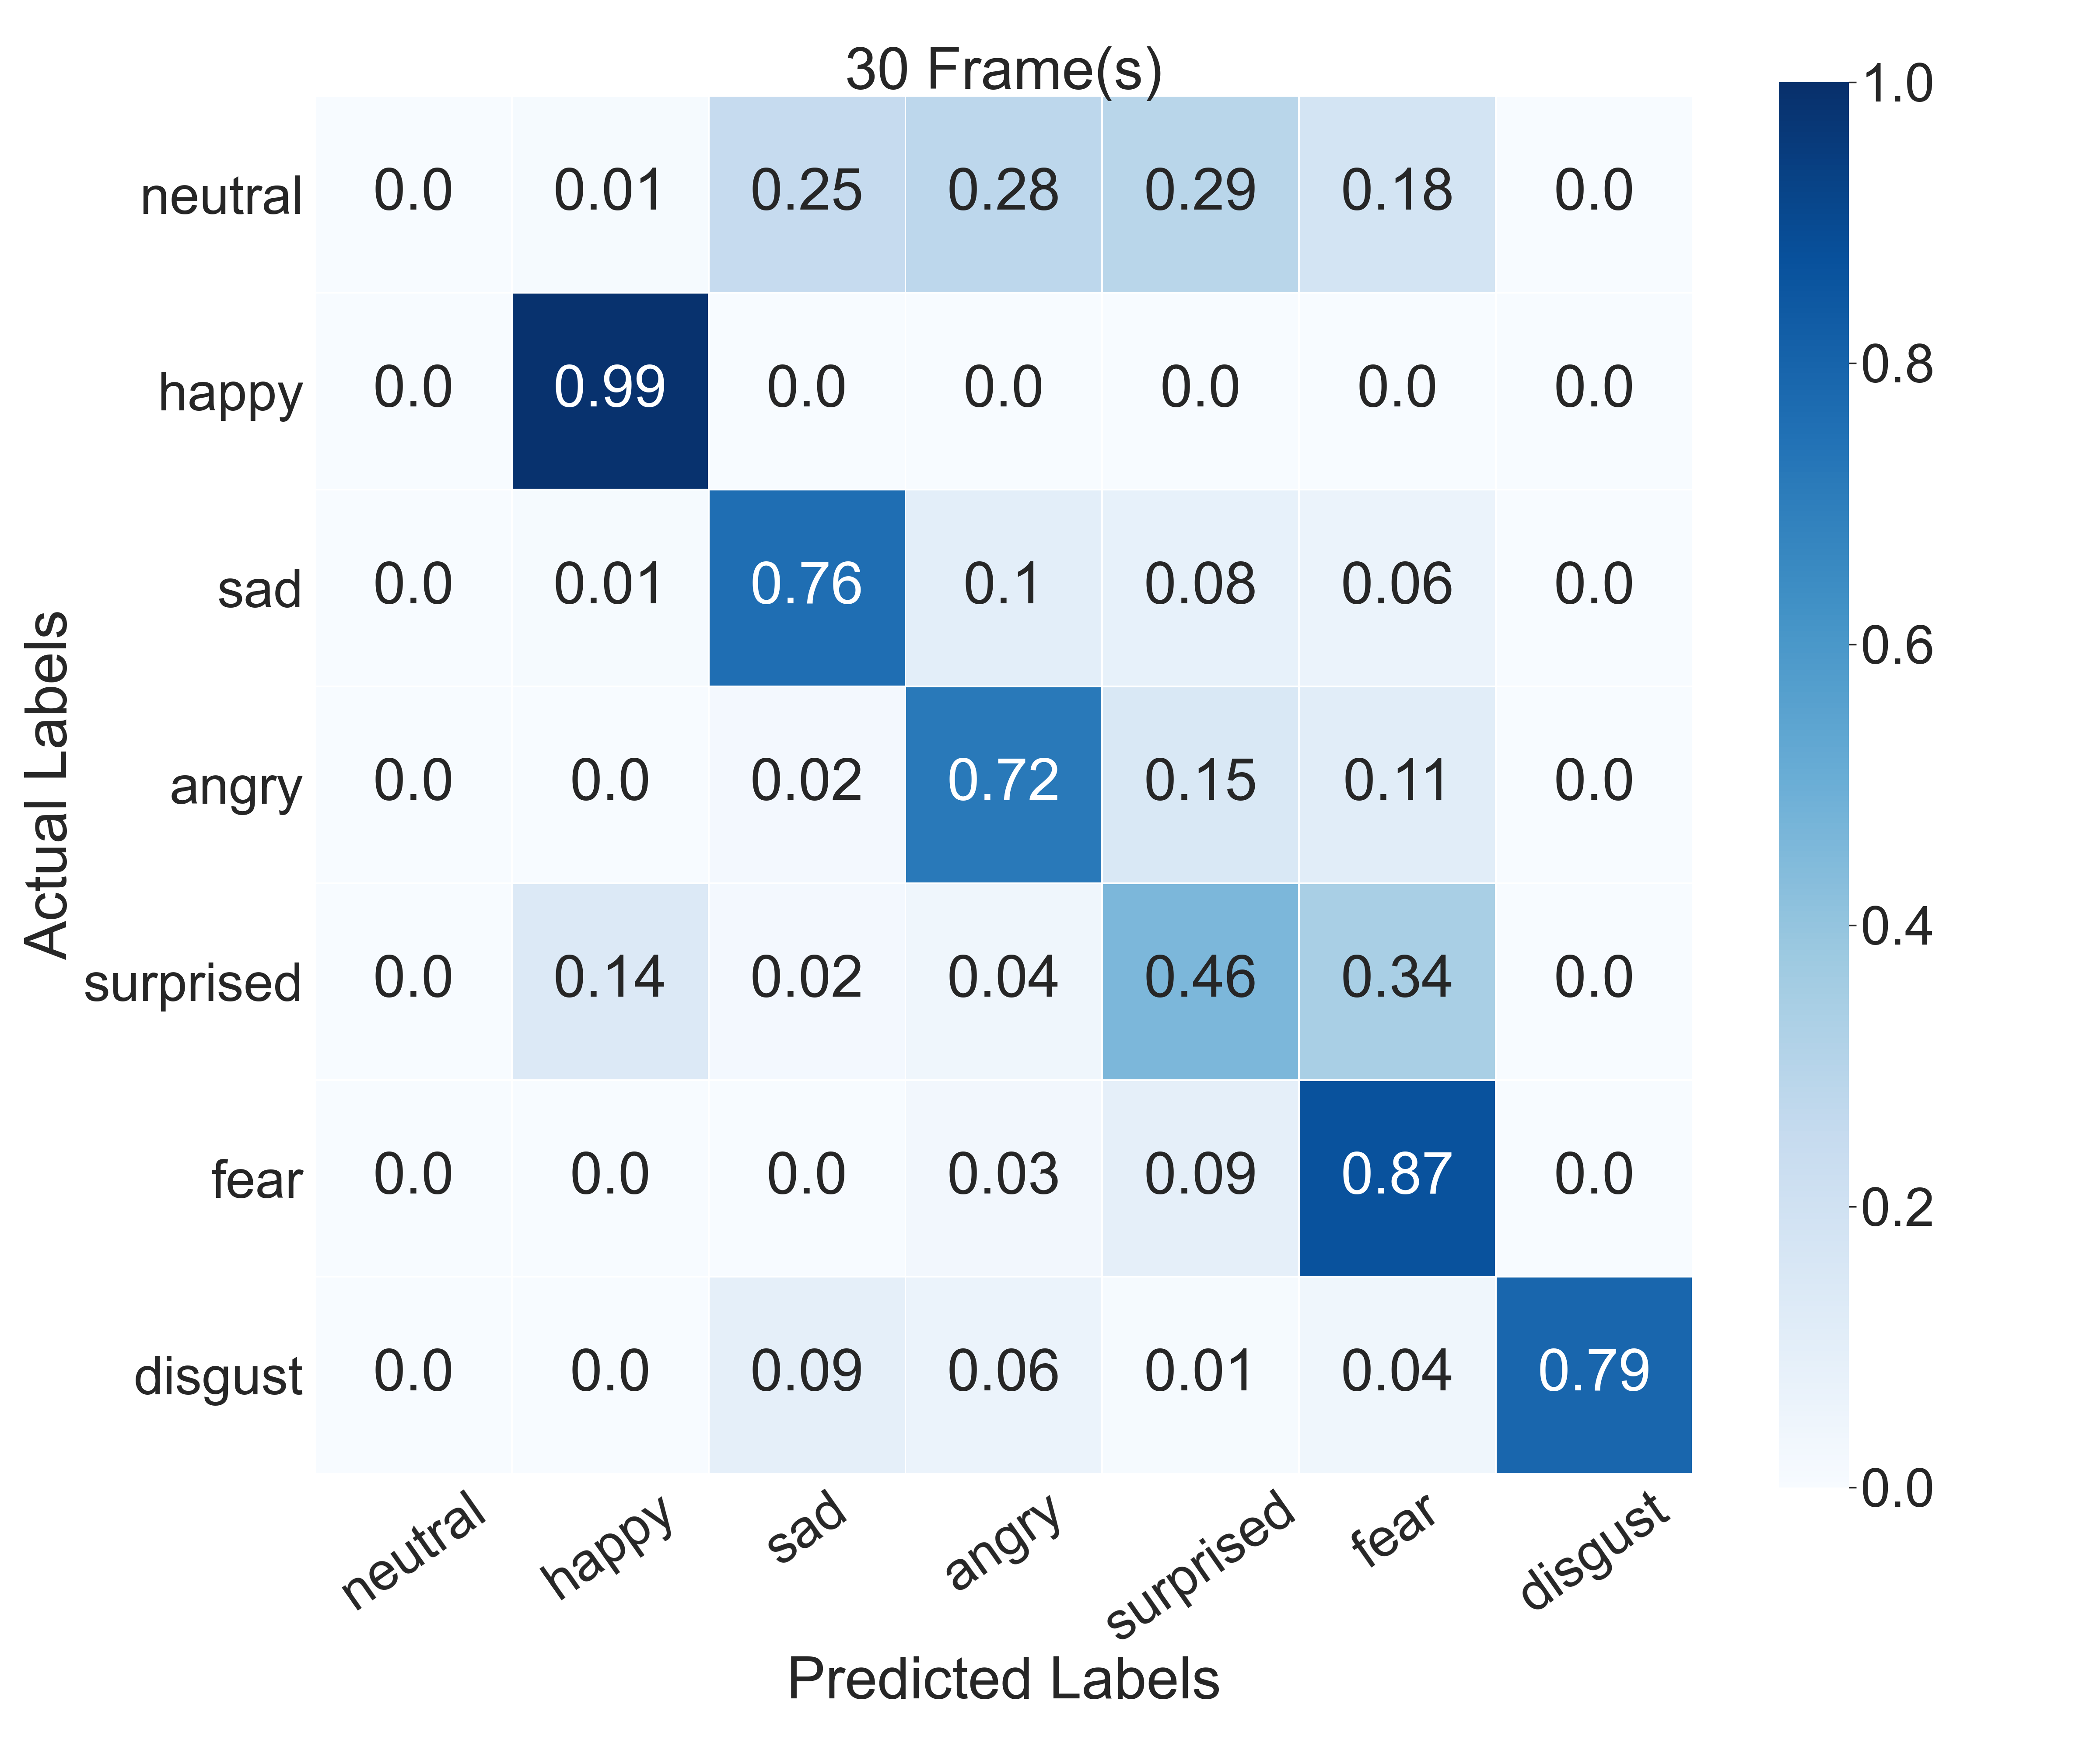
\includegraphics[width=\textwidth]{res/conf_busso_30.png}
    \end{subfigure}
    \begin{subfigure}[b]{0.45\textwidth}
      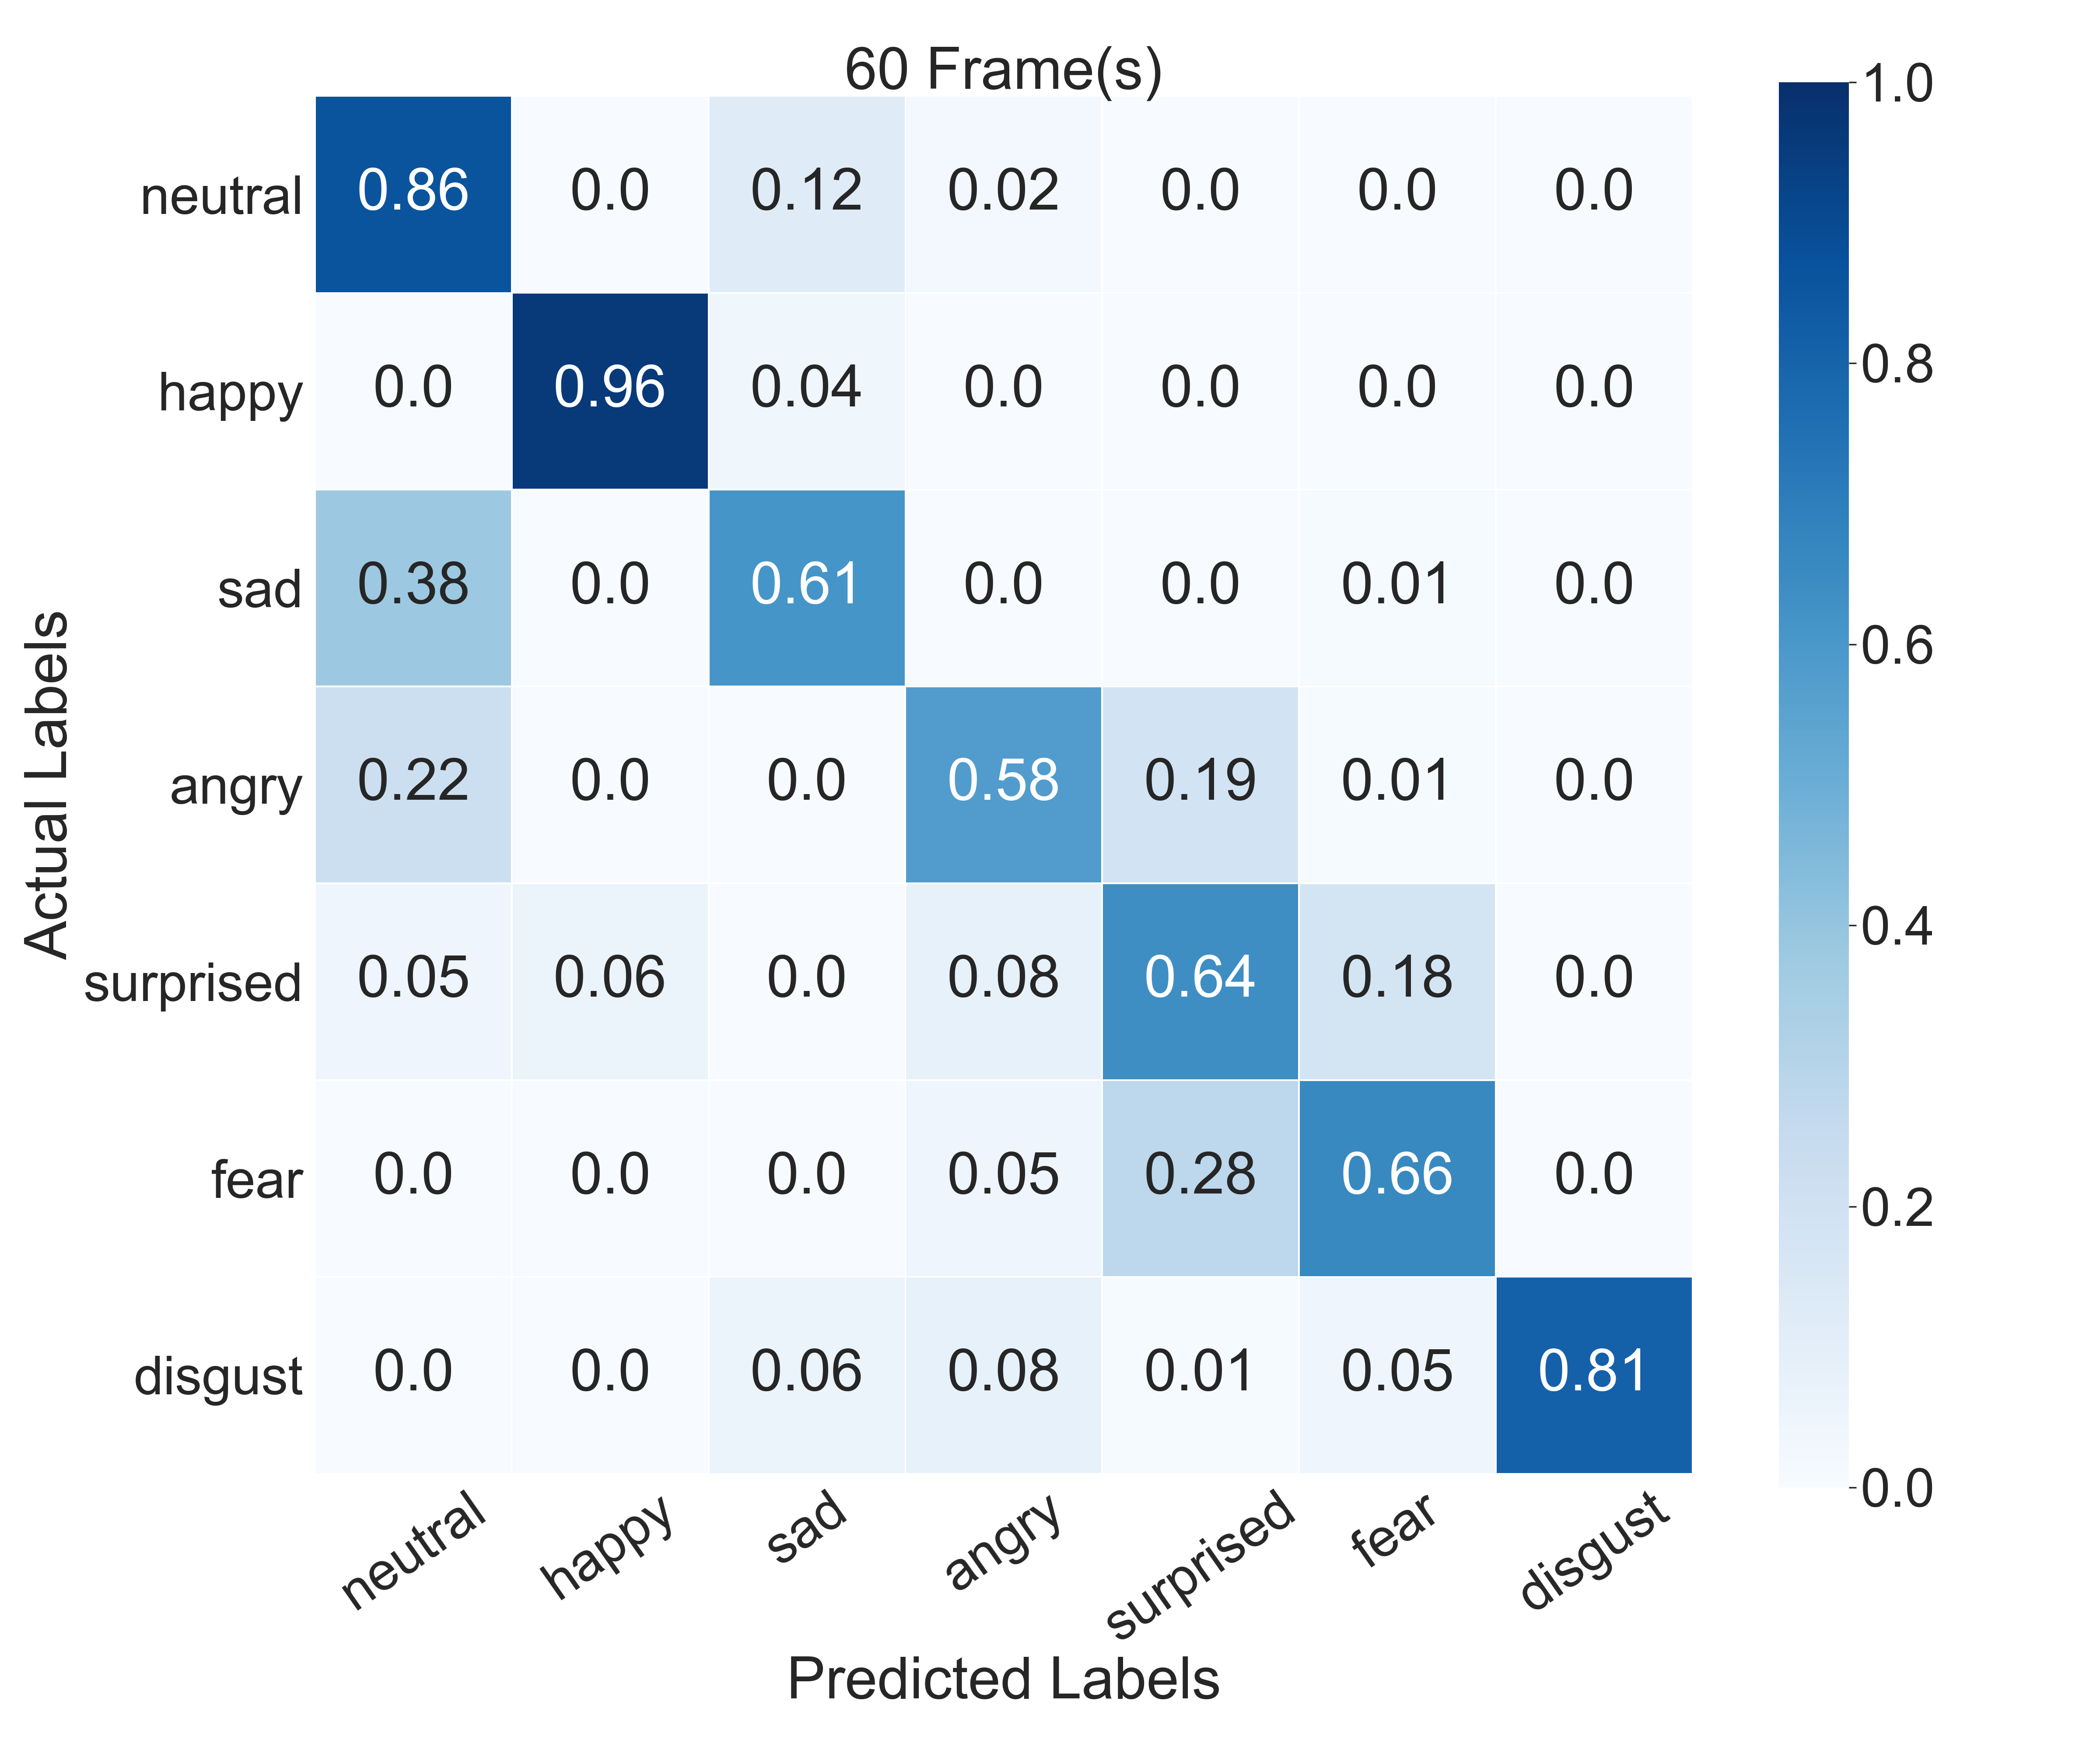
\includegraphics[width=\textwidth]{res/conf_busso_60.png}
    \end{subfigure}
    \begin{subfigure}[b]{0.45\textwidth}
      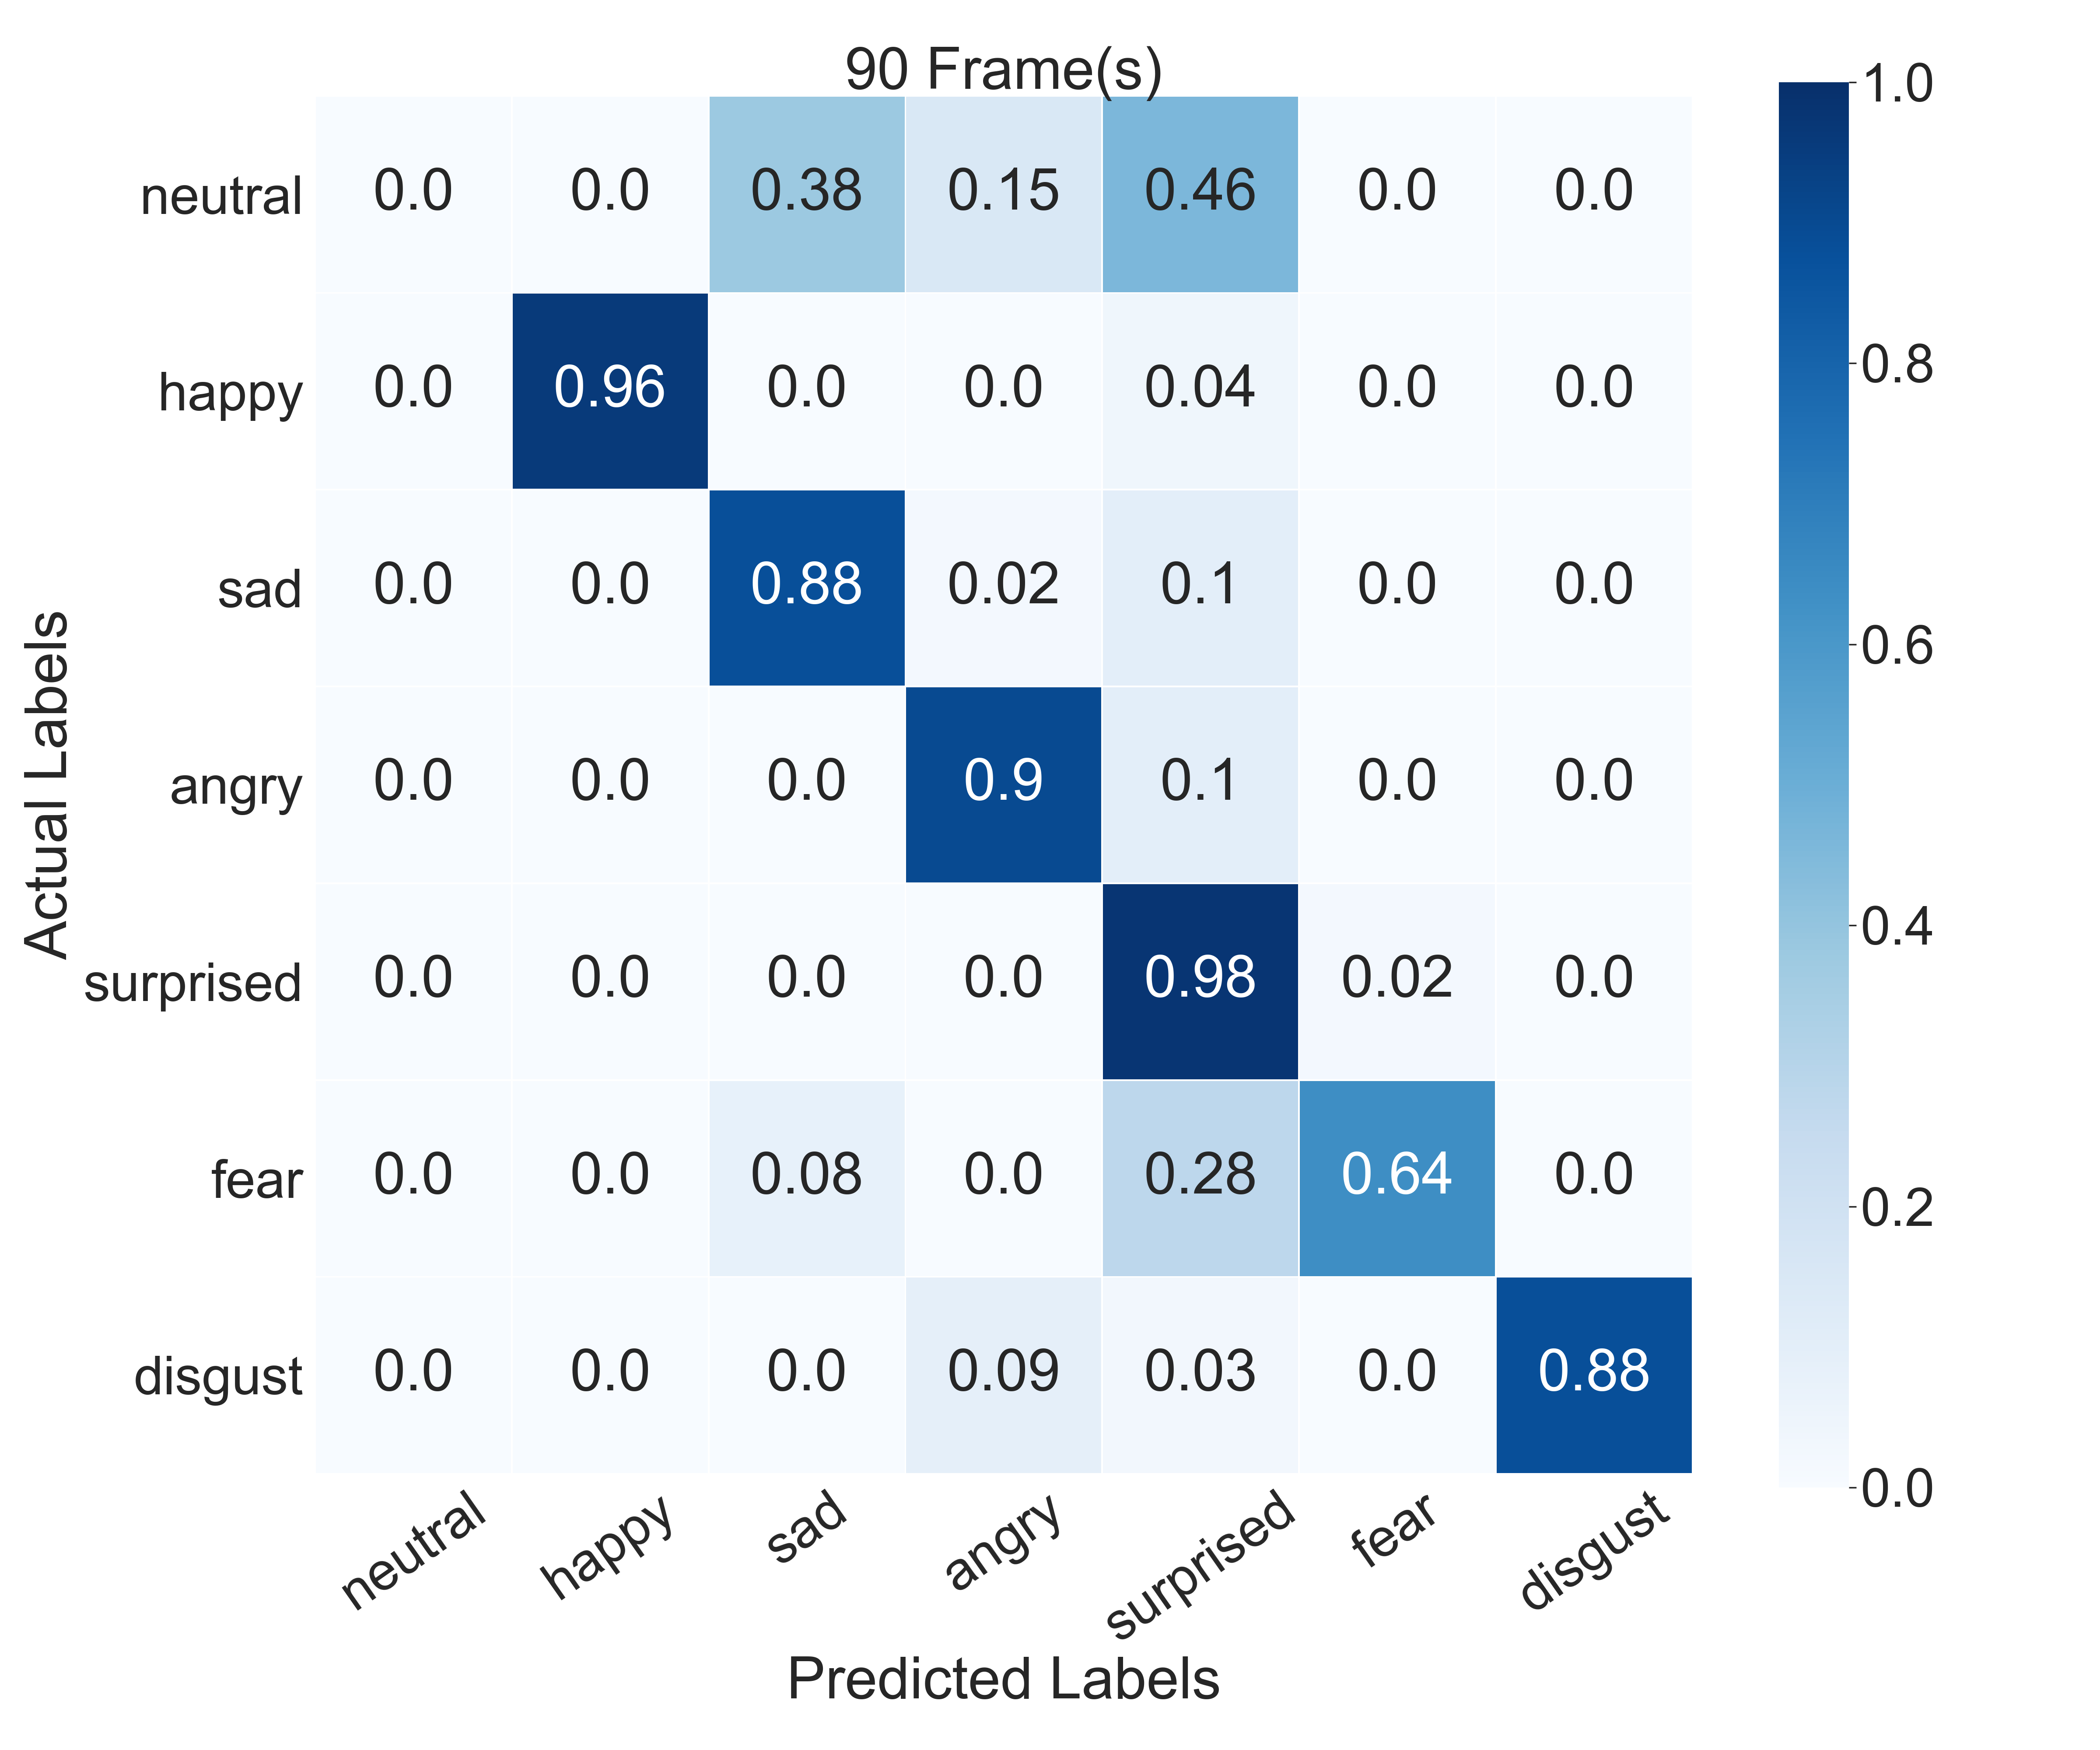
\includegraphics[width=\textwidth]{res/conf_busso_90.png}
    \end{subfigure}
    \caption{Confusion matrices of the validation data for the Style Extractor fusion model.}
    \label{fig:lipnet_conf}
\end{figure}


Confusion matrices allow us to take a deeper look into the model performance. Figure \ref{fig:fer_conf} shows the confusion matrices of the model without any lexical compensator through all frame-window sizes. We notice a consistent overfitting towards \texttt{neutral} labels in all temporal settings. There also remain significant mislabels around \texttt{surprised} labels on models with 1, 30, and 60 frames. At 90 frames, the model becomes very robust on all other emotions except for the overfitting towards \texttt{neutral}.

The confusion matrices for the LipNet model in figure \ref{fig:lipnet_conf} similarly show an improvement along the temporal dimension. A similar overfit towards \texttt{neutral} persists throughout. However at 90 frames, the LipNet model does not manage to alleviate the issues surrounding false \texttt{surprised} labels. The overfit on \texttt{surprised} was indeed lower on the single frame model. This might however be explained by the very severe overlabelling on \texttt{neutral} labels in that model.

A different pattern emerges on the model using our own style extractor. The \texttt{neutral} label is ignored by the model, except when trained on 60 frames. The \texttt{surprised} emotion has a notably worse performance compared to the other emotions, which can be explained by the lack of surprised videos in the CREMA-D dataset used to train the style extractor.
% TODO: epochs -> best result after 4-7 epochs

\subsection{Cross Dataset Validation}
All our models on the FER section were trained on RAVDESS. An interesting question is if and how well the models generalize to other datasets, in this case CREMA-D.

\subsection{Phonetic (In-)Dependence}
In section \ref{sec:human} we already saw that the phonetic performance of existing FER models was low and varied between phonemes. After training our single-frame models, we run the same analysis again to determine the improvements in phonetic performance and to figure out if and how the lexical compensators improve the results.
\subsection{Multilingual Datasets}
In section \ref{sec:german} we collected samples for a German dataset. We now want to analyse the performance of our models to draw conclusions on their multilingual performance.

% \subsection{Performance on Non-talking Subjects}
